\newpage
\section{模型的建立与求解}

\subsection{问题一的模型建立与求解}
\subsubsection{具体分析}

问题一要求在销售量、亩产量、种植成本、销售价格均不随年份变化的确定性口径下，制定2024--2030年共7年的最优种植方案，属多约束组合优化问题。核心难点在于：(i) 54块地块需按地块类型与季次匹配可种作物；(ii) 需满足水浇地第二季复种、重茬回避、豆类三年轮作等农业制度约束；(iii) 每作物季次的产量不得超过预期销售量上限。由于单作物种植面积以整块地计（每地块每季只能种一种作物），决策变量天然为0-1整数，故采用0-1整数线性规划（MILP）建模\cite{rotmilp2024,veglp2019,cumc2026}，并分别考察"超产滞销"（情形1）与"超产按50\%降价出售"（情形2）两种销售规则。

\begin{figure}[htbp]
	\centering
	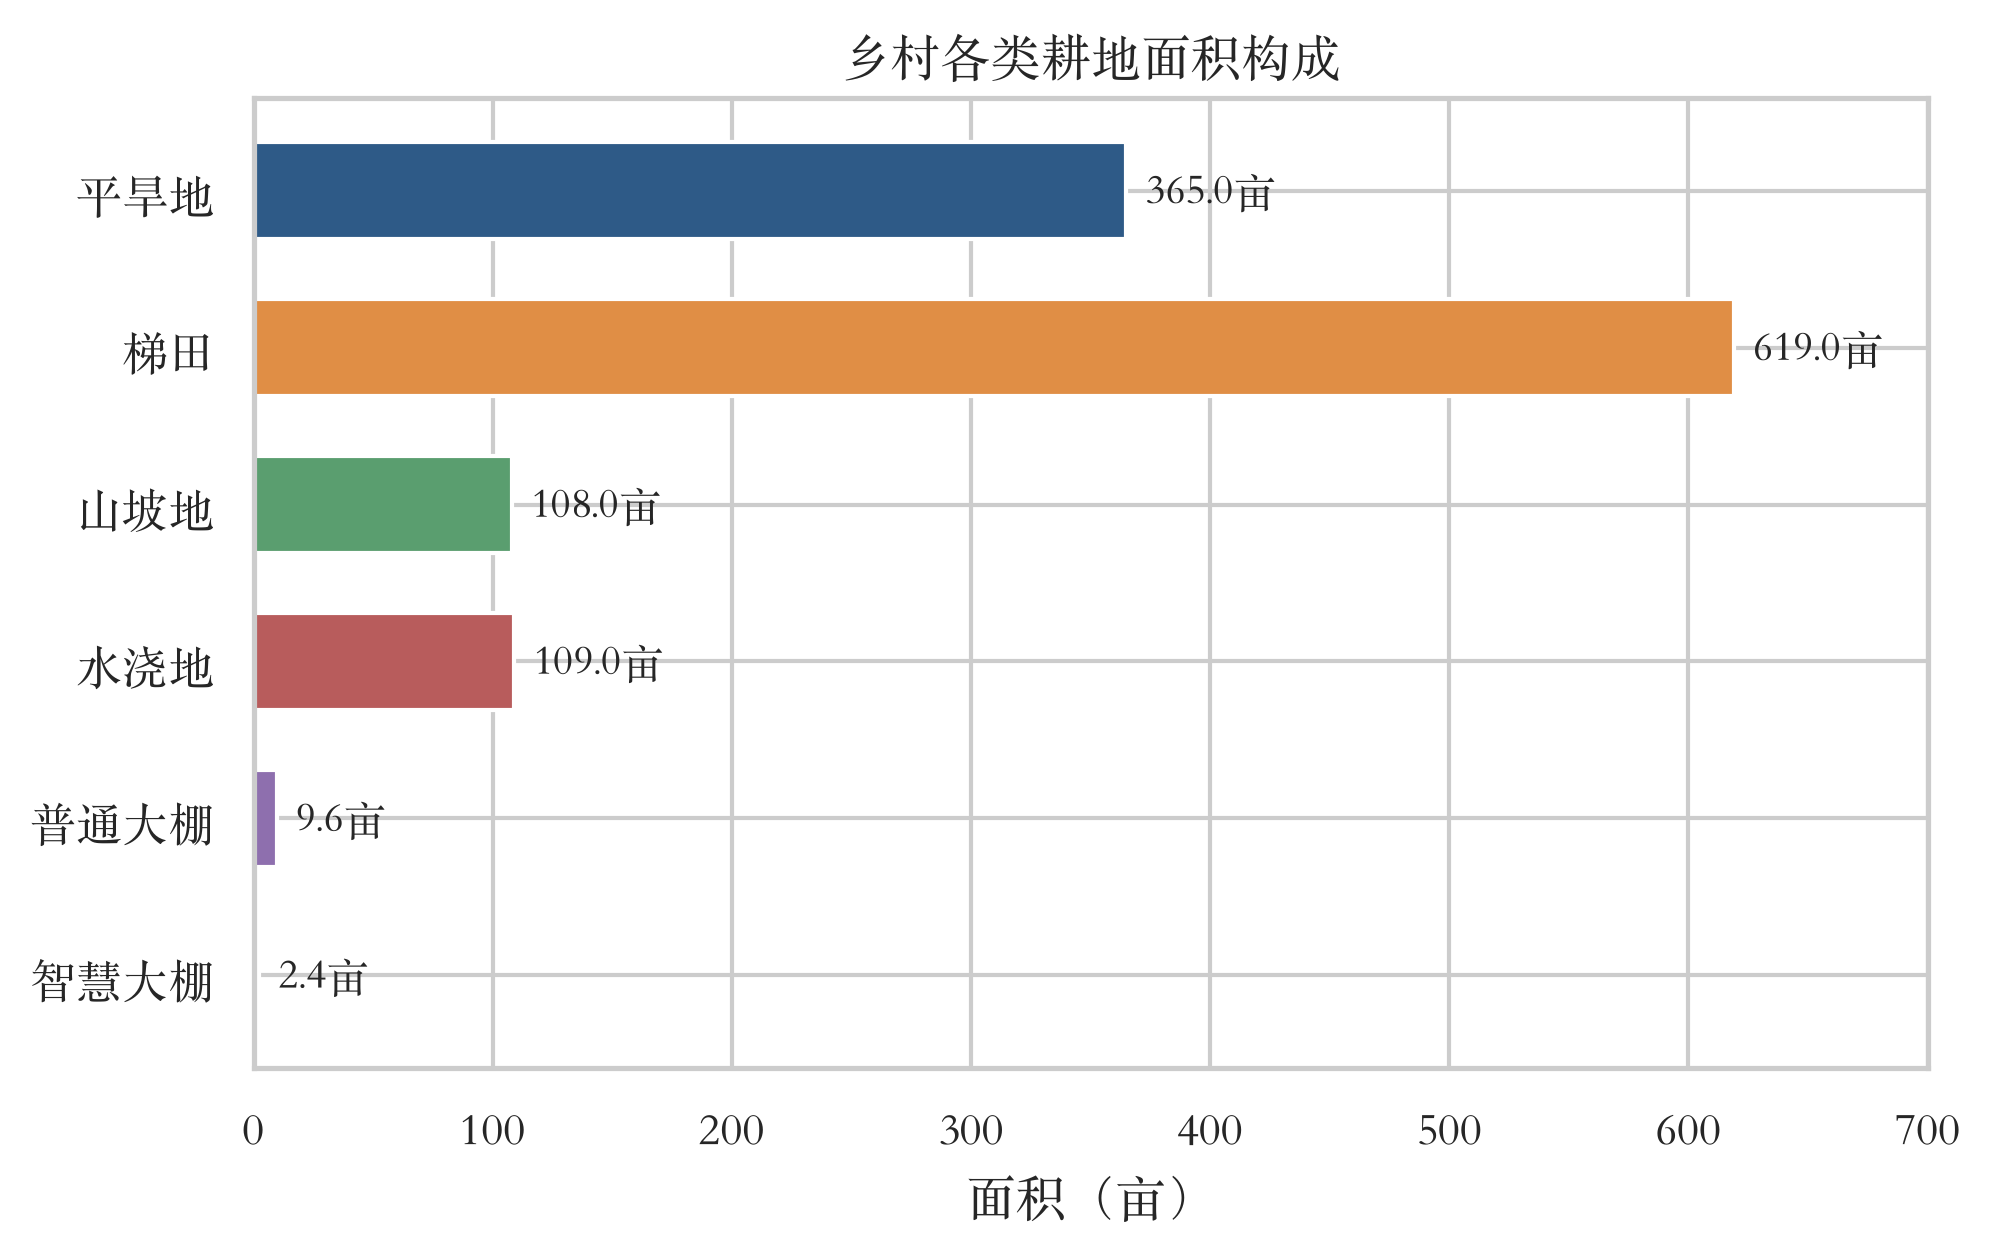
\includegraphics[width=0.78\textwidth]{figures/fig_land_structure.png}
	\caption{地块结构与2023年利用情况}
	\label{fig:land-structure}
\end{figure}

\subsubsection{模型准备}

附件1中2023年种植表存在合并单元格与部分地块当季未种的情况，经前向填充与数值清洗后，得到54地块、41作物、两季次的完整种植结构，如图~\ref{fig:land-structure} 所示。由图可见，平旱地、梯田、山坡地以小麦、玉米及豆类粮食为主，水浇地第一季种植水稻、第二季复种大白菜等蔬菜，普通大棚与智慧大棚种植蔬菜与食用菌。

各作物2023年实际产量即作为其预期销售量的基准 $S_{c,s}$；各作物在各地块的亩产量 $y_{c,p,s}$、种植成本 $c_{c,p,s}$ 与销售单价 $r_{c,s}$ 均取自附件并作如下处理：单价为区间型数据时取区间中点；售价有批发价与市场价之分的，统一采用市场价口径。经统计，按2023年实际种植结构核算的当年总净收益约 $592.6$ 万元（见模型求解部分）。

\subsubsection{模型建立}

\textbf{(1) 决策变量}

\begin{equation}
x_{p,t,s,c} = \begin{cases} 1, & \text{地块 } p \text{ 第 } t \text{ 年第 } s \text{ 季种植作物 } c\\ 0, & \text{否则} \end{cases}
\end{equation}

其中 $p\in\mathcal{P}$，$t\in\mathcal{T}=\{2024,\ldots,2030\}$，$s\in\{\text{第一季},\text{第二季}\}$，$c\in\mathcal{C}_{ps}$。只有 $S_{c,s}>0$（即有2023年销售基准）的作物季次组合才进入变量集合。

\textbf{(2) 目标函数（情形1：超产滞销）}

情形1下，超出预期销售量 $S_{c,s}$ 的产量无法售出、不计收益，故第 $t$ 年作物 $c$ 季次 $s$ 的收益为 $\min(\text{产量},S_{c,s})\cdot r_{c,s}$。由于 $S_{c,s}$ 为常数、销售量为线性，目标函数可写为

\begin{equation}
\max\quad \sum_{p,t,s,c}\big( r_{c,s} y_{c,p,s} - c_{c,p,s} \big) A_p\, x_{p,t,s,c}
\label{eq:obj1}
\end{equation}

\textbf{(3) 约束条件}

\begin{align}
& \sum_{c\in\mathcal{C}_{ps}} x_{p,t,s,c} \le 1, && \forall p,\ t,\ s \label{eq:c1}\\
& \sum_{c\in\{35,36,37\}} x_{p,t,\text{二},c} + x_{p,t,\text{一},\text{水稻}} = 1, && \forall p\in\mathcal{P}_D,\ t \label{eq:c2}\\
& x_{p,t,s,c} + x_{p,t+1,s,c} \le 1, && \forall p,\ s,\ c,\ t \label{eq:c3}\\
& \sum_{t\in\{w,w+1,w+2\}}\sum_{s}\sum_{c\in\mathcal{C}^b} x_{p,t,s,c} \ge 1 - b_{p,w}, && \forall p,\ w\in\{2023,\ldots,2028\} \label{eq:c4}\\
& \sum_{p} A_p\, y_{c,p,s}\, x_{p,t,s,c} \le S_{c,s}, && \forall (c,s),\ t \label{eq:c5}
\end{align}

其中，式(\ref{eq:c1})为土地容量约束，保证每地块每季至多种植一种作物（单作满块）；式(\ref{eq:c2})为水浇地结构约束，第二季复种蔬菜数与第一季是否种水稻之和恒为1，即"种水稻则不种二季菜，不种水稻则二季复种一种菜"；式(\ref{eq:c3})为重茬约束，同一地块相邻两年同一季次不得种植同一种作物；式(\ref{eq:c4})为豆类轮作约束，对任意滚动三年窗口（含2023年已种植数据，$b_{p,w}$为2023年窗口起始时的已知豆类指示）至少种植一次豆类作物；式(\ref{eq:c5})为销售上限约束，各作物各季次年产量不超过预期销售量。对情形1，当单个地块产量已超过总销售上限时，该地块种植该作物的组合在最优解中必不可行，建模时预先剔除以缩减规模。

\textbf{(4) 情形2（超产按50\%降价）}

引入原价售出量 $u_{c,s,t}$ 与折价售出量 $v_{c,s,t}$，二者满足 $u+v=\text{产量}$、$u\le S_{c,s}$，目标变为

\begin{equation}
\max\quad \sum_{c,s,t}\big( r_{c,s} u_{c,s,t} + 0.5\,r_{c,s} v_{c,s,t} \big) - \sum_{p,t,s,c} c_{c,p,s} A_p x_{p,t,s,c}
\label{eq:obj2}
\end{equation}

情形2允许超产部分按半价出售，因此方案会更倾向于扩大高收益作物的种植面积，销售上限的约束作用被部分放松。

\subsubsection{模型求解}

该模型为含约6800个0-1变量、上万条约束的大规模整数规划，采用分支定界框架求解。本文使用基于 Python 的 HiGHS 求解器（\texttt{scipy.optimize.milp}）求解，设置相对最优间隙（MIP gap）$1\%$，单情形求解时间上限15分钟；求解环境为 macOS + Python 3.14，多核并行。

两种情形的最优方案见附录输出表及图~\ref{fig:plan-q1-1}。求解结果汇总如下：情形1（超产滞销）2024--2030年总净收益约 $\textbf{3{,}988{,}2}$ 万元，情形2（超产按50\%折价）约 $\textbf{5{,}918{,}0}$ 万元，后者较前者提高约48.4\%，相对间隙均控制在1\%以内。

\subsubsection{问题一结果分析}

\begin{figure}[htbp]
	\centering
	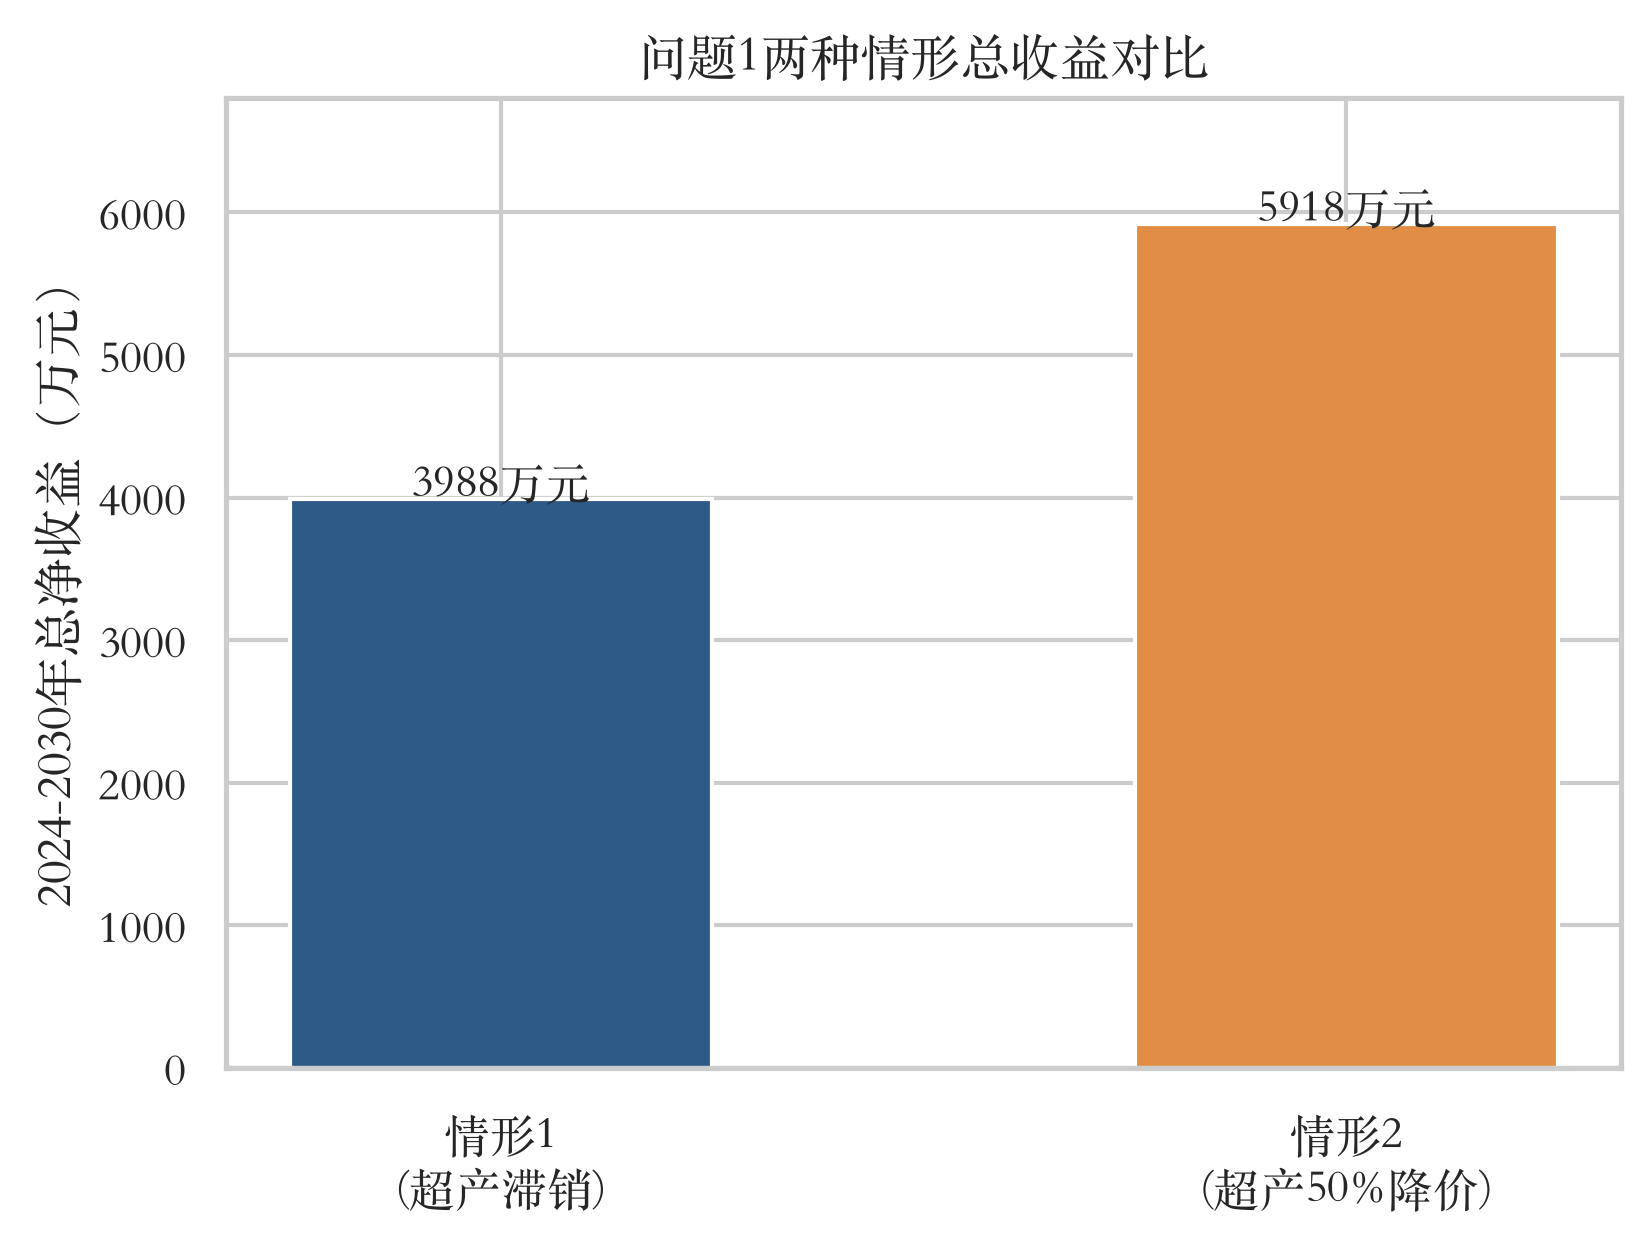
\includegraphics[width=0.68\textwidth]{figures/fig_cases_compare.png}
	\caption{两种情形总收益对比}
	\label{fig:cases-compare}
\end{figure}

\begin{figure}[htbp]
	\centering
	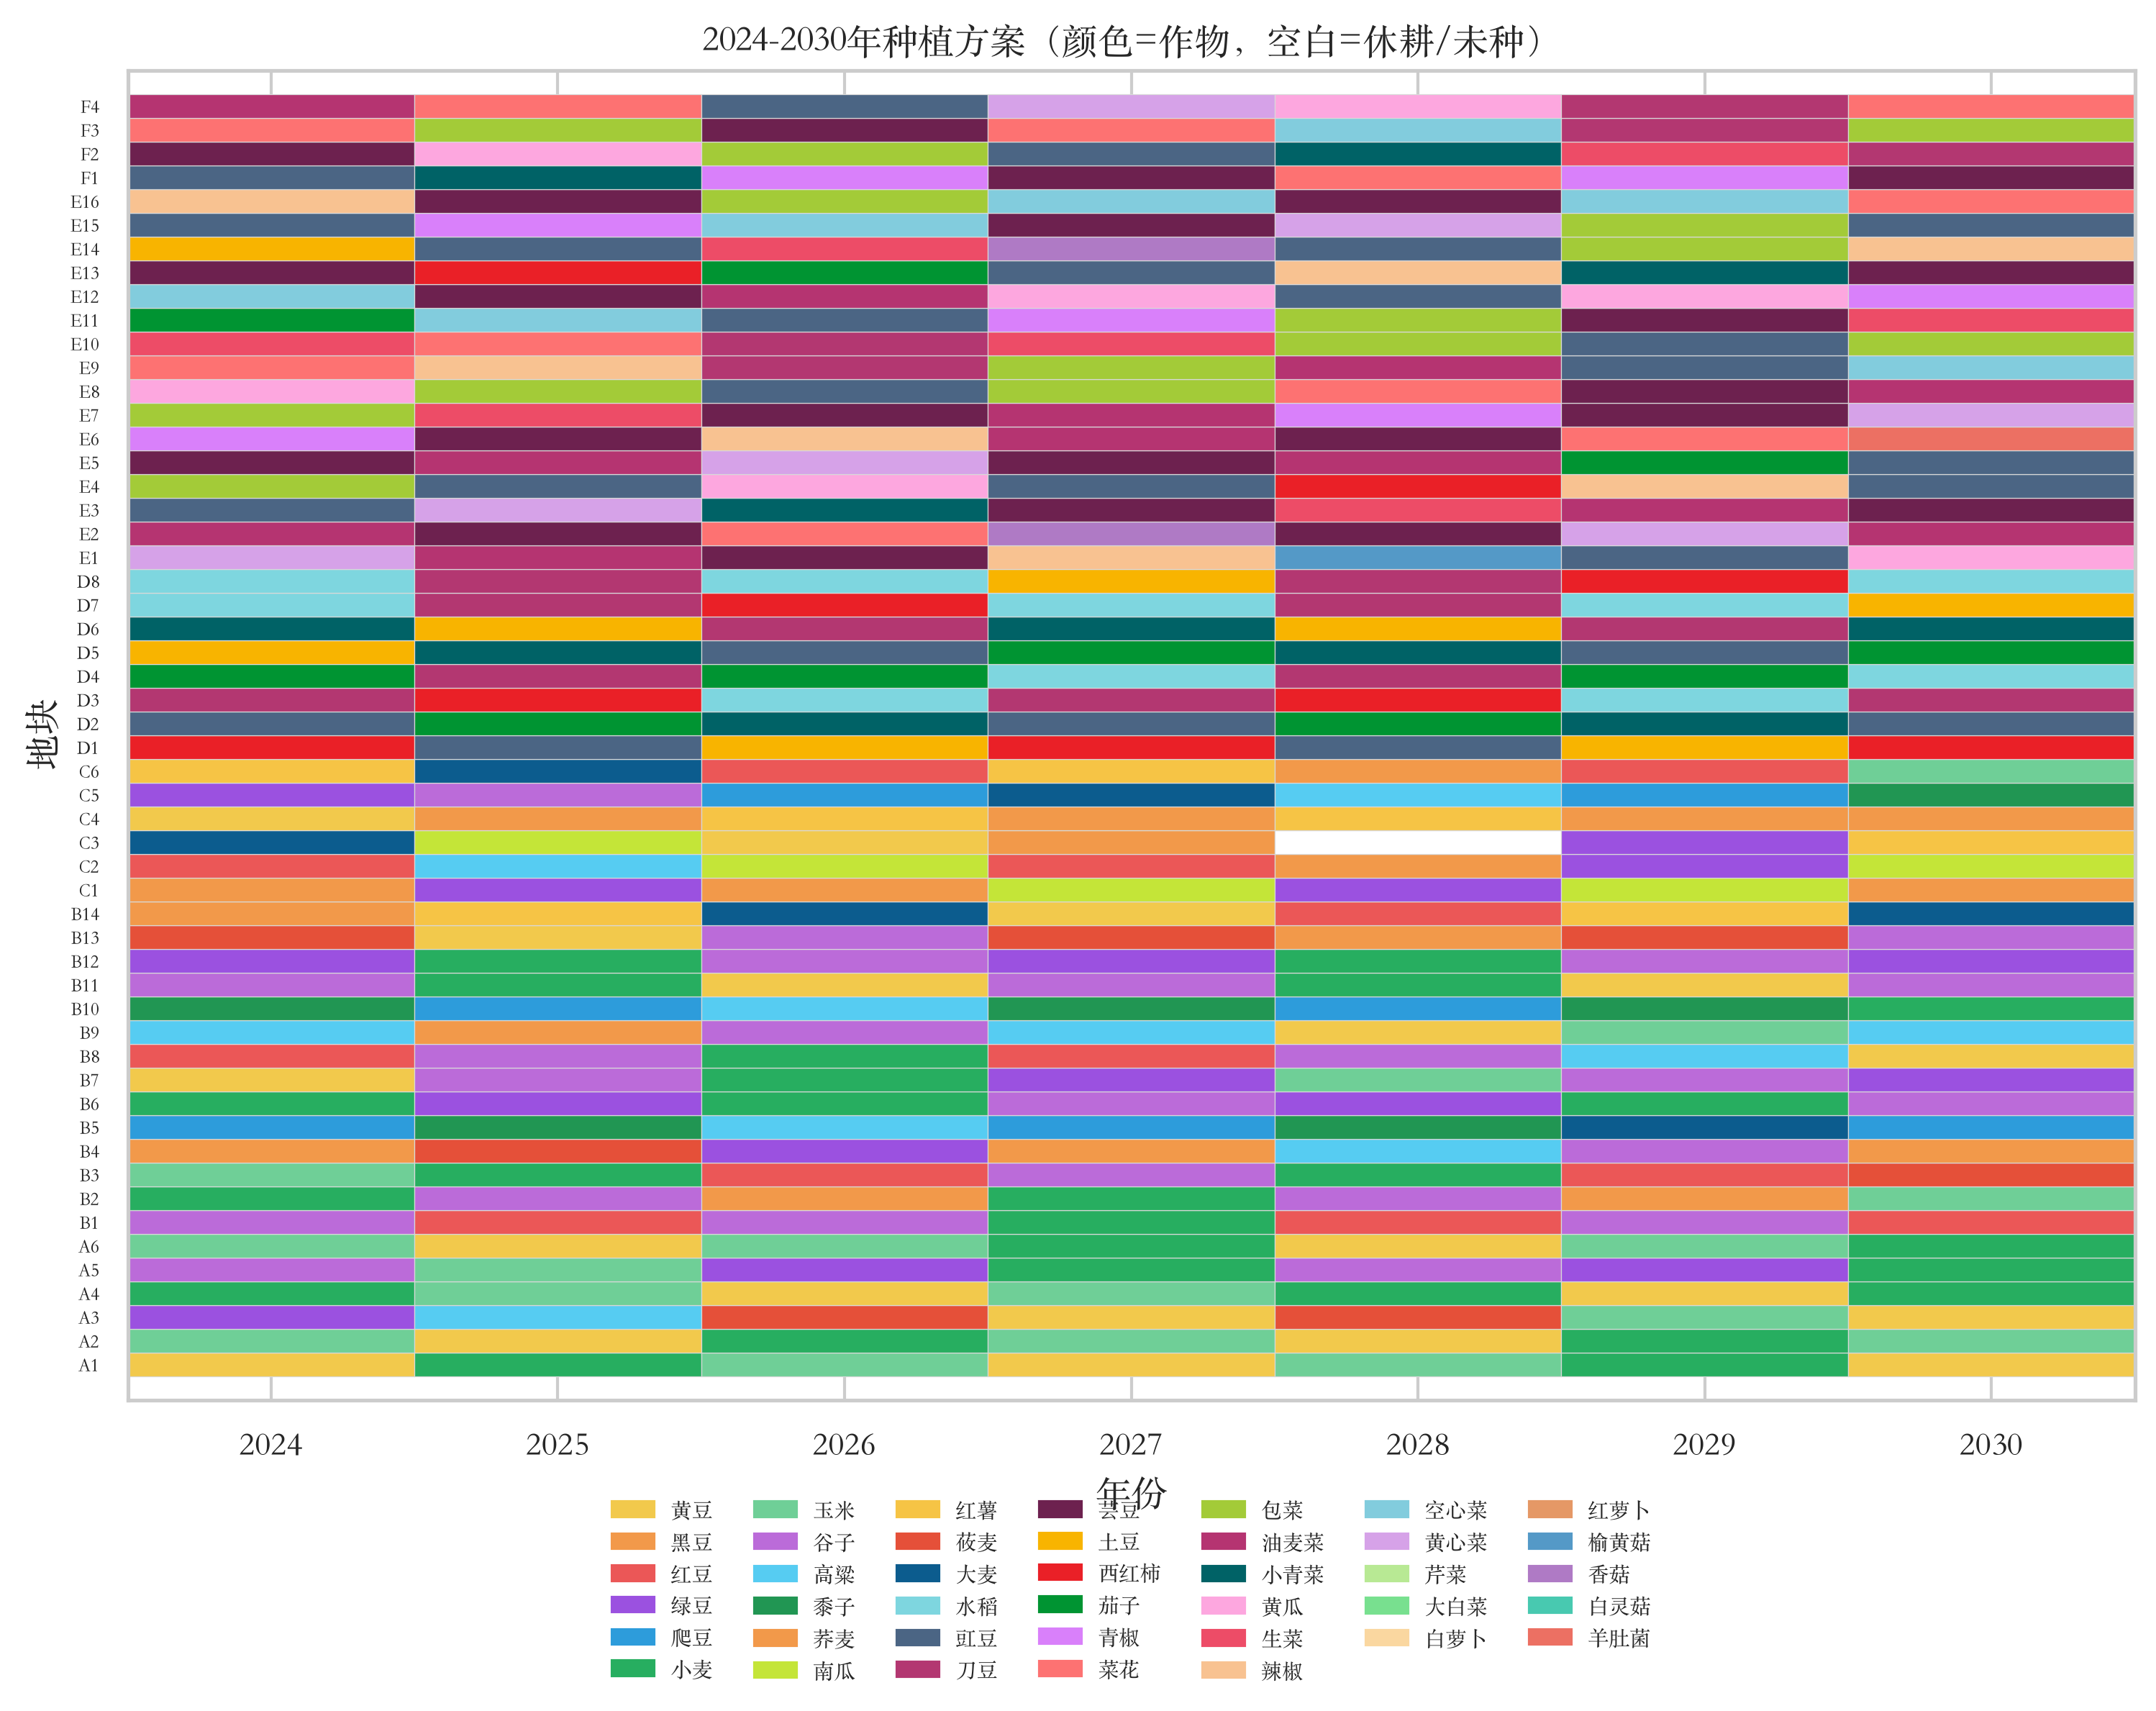
\includegraphics[width=0.78\textwidth]{figures/fig_plan_q1_1.png}
	\caption{情形1最优种植方案热图}
	\label{fig:plan-q1-1}
\end{figure}

\begin{figure}[htbp]
	\centering
	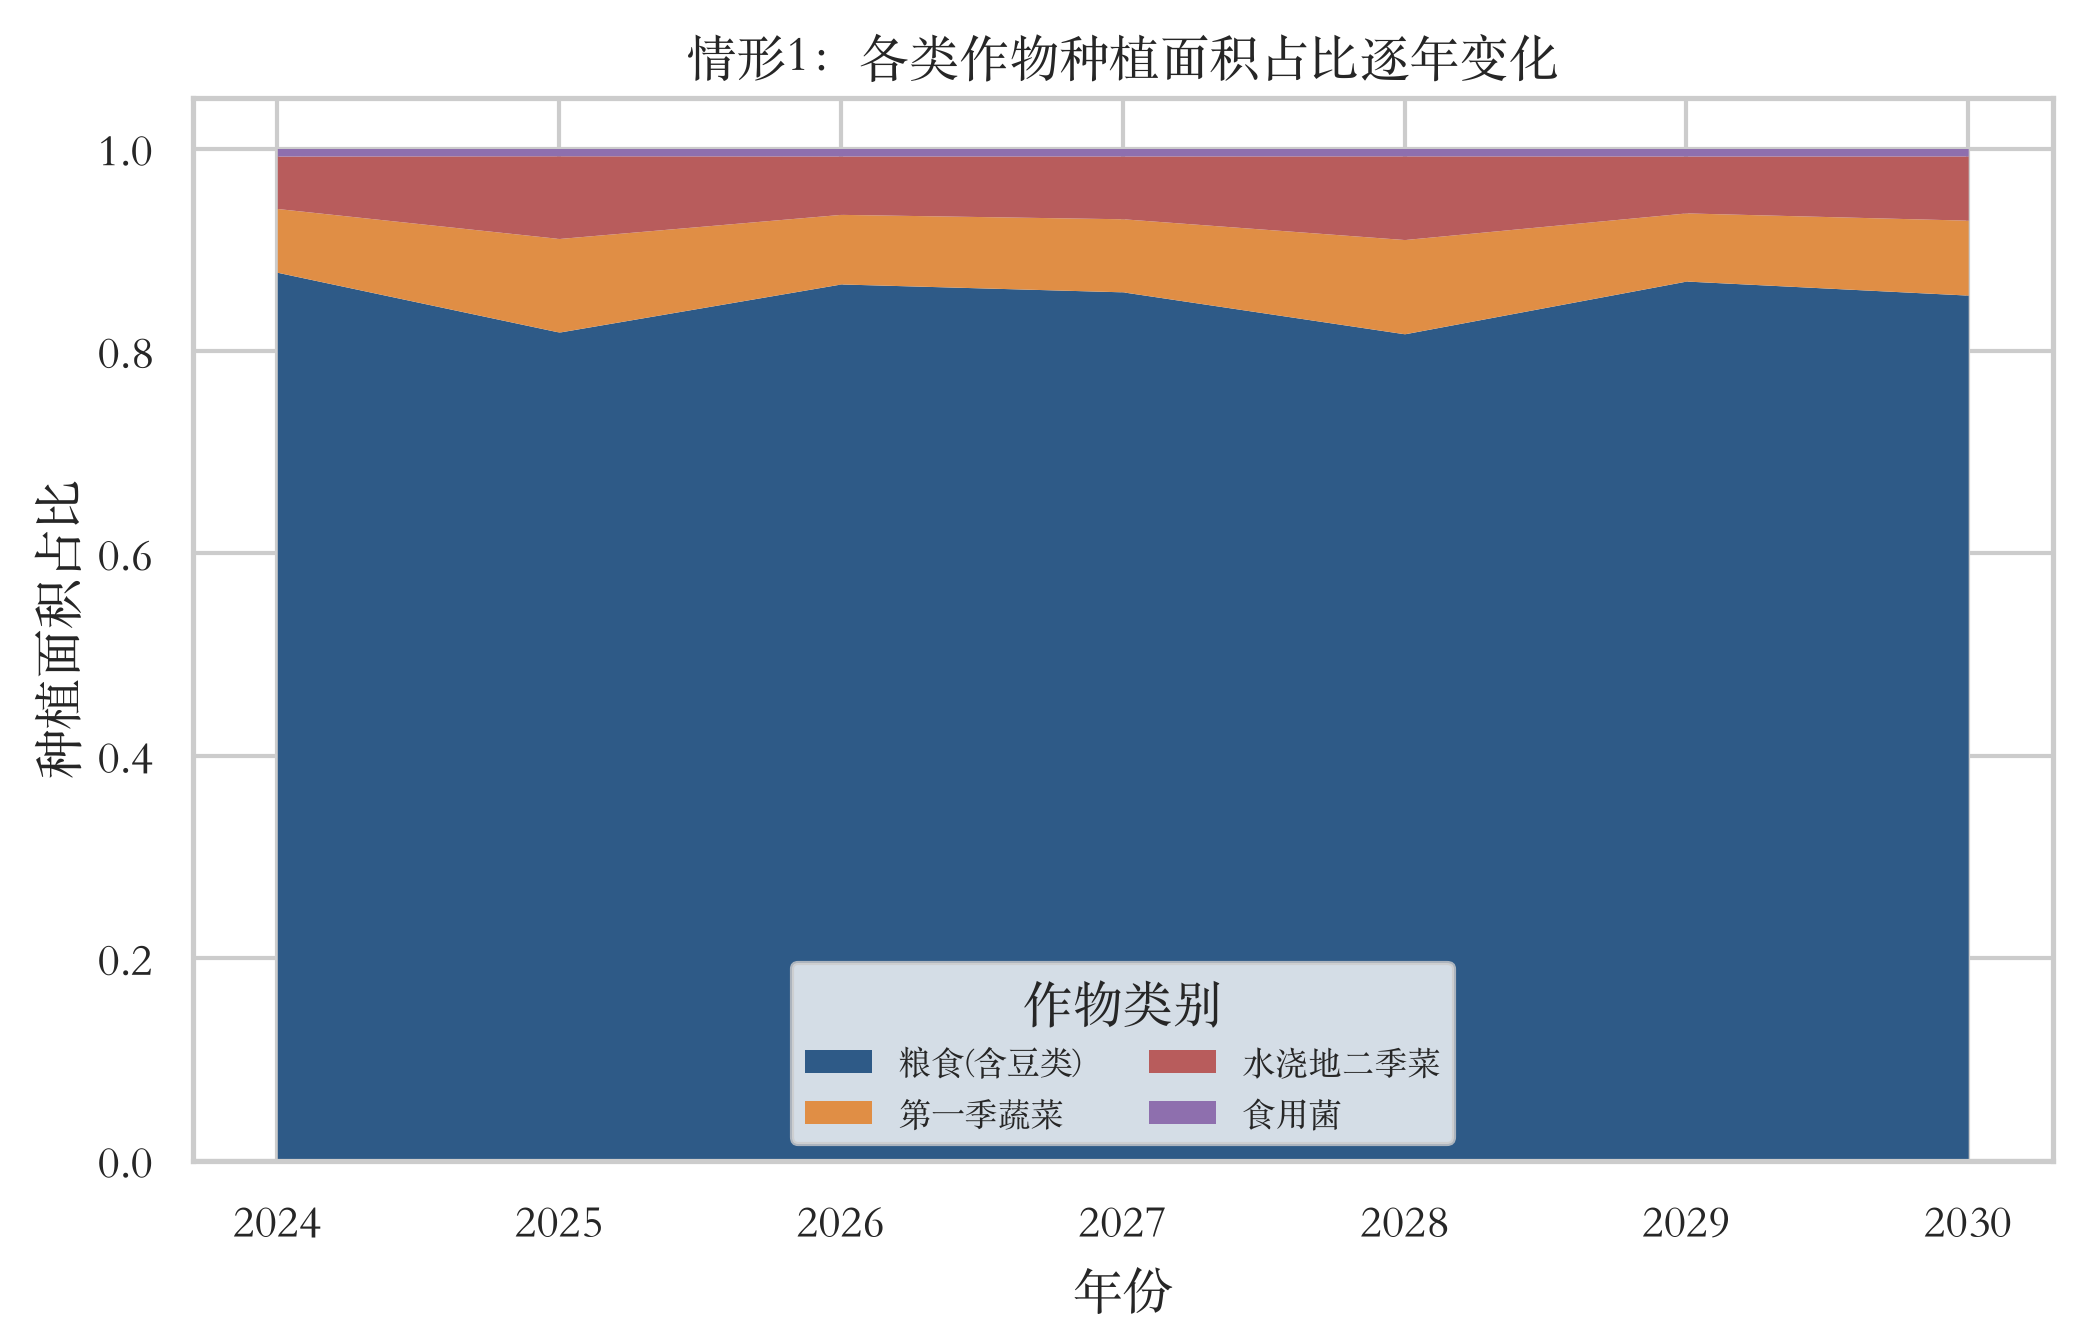
\includegraphics[width=0.68\textwidth]{figures/fig_area_share_q1_1.png}
	\caption{情形1各类作物种植面积占比变化}
	\label{fig:area-share-q1-1}
\end{figure}

情形1下，如图~\ref{fig:cases-compare} 所示，2024--2030年总净收益为 $\textbf{3{,}988{,}2}$ 万元。由图~\ref{fig:plan-q1-1} 与图~\ref{fig:area-share-q1-1} 可见，种植结构以粮食为主：平旱地、梯田、山坡地普遍种植小麦、谷子、玉米与黄豆、绿豆等豆类，粮食类面积占比由2023年的87.5\%微调至2024年的87.8\%、2030年的85.5\%，蔬菜占比由11.8\%小幅升至13.8\%。这是因为情形1下各作物季次产量不得超过预期销售量，超产即滞销浪费，故模型倾向于把销售上限较大、价格相对稳定的粮食作物作为主栽品种；同时豆类三年轮作约束使黄豆、绿豆、红豆等豆类作物在各地块间有序轮换（图中豆类在各年份的地块分布呈明显轮换规律）。受整块地种植粒度与水浇地第二季复种制度的限制，个别小销量蔬菜（如红萝卜、刀豆）出现结构性超产，全周期总产量中超产滞销约11.2\%，这是复种制度约束下难以完全避免的浪费，模型已通过调整种植组合将其降至最低。

\begin{figure}[htbp]
	\centering
	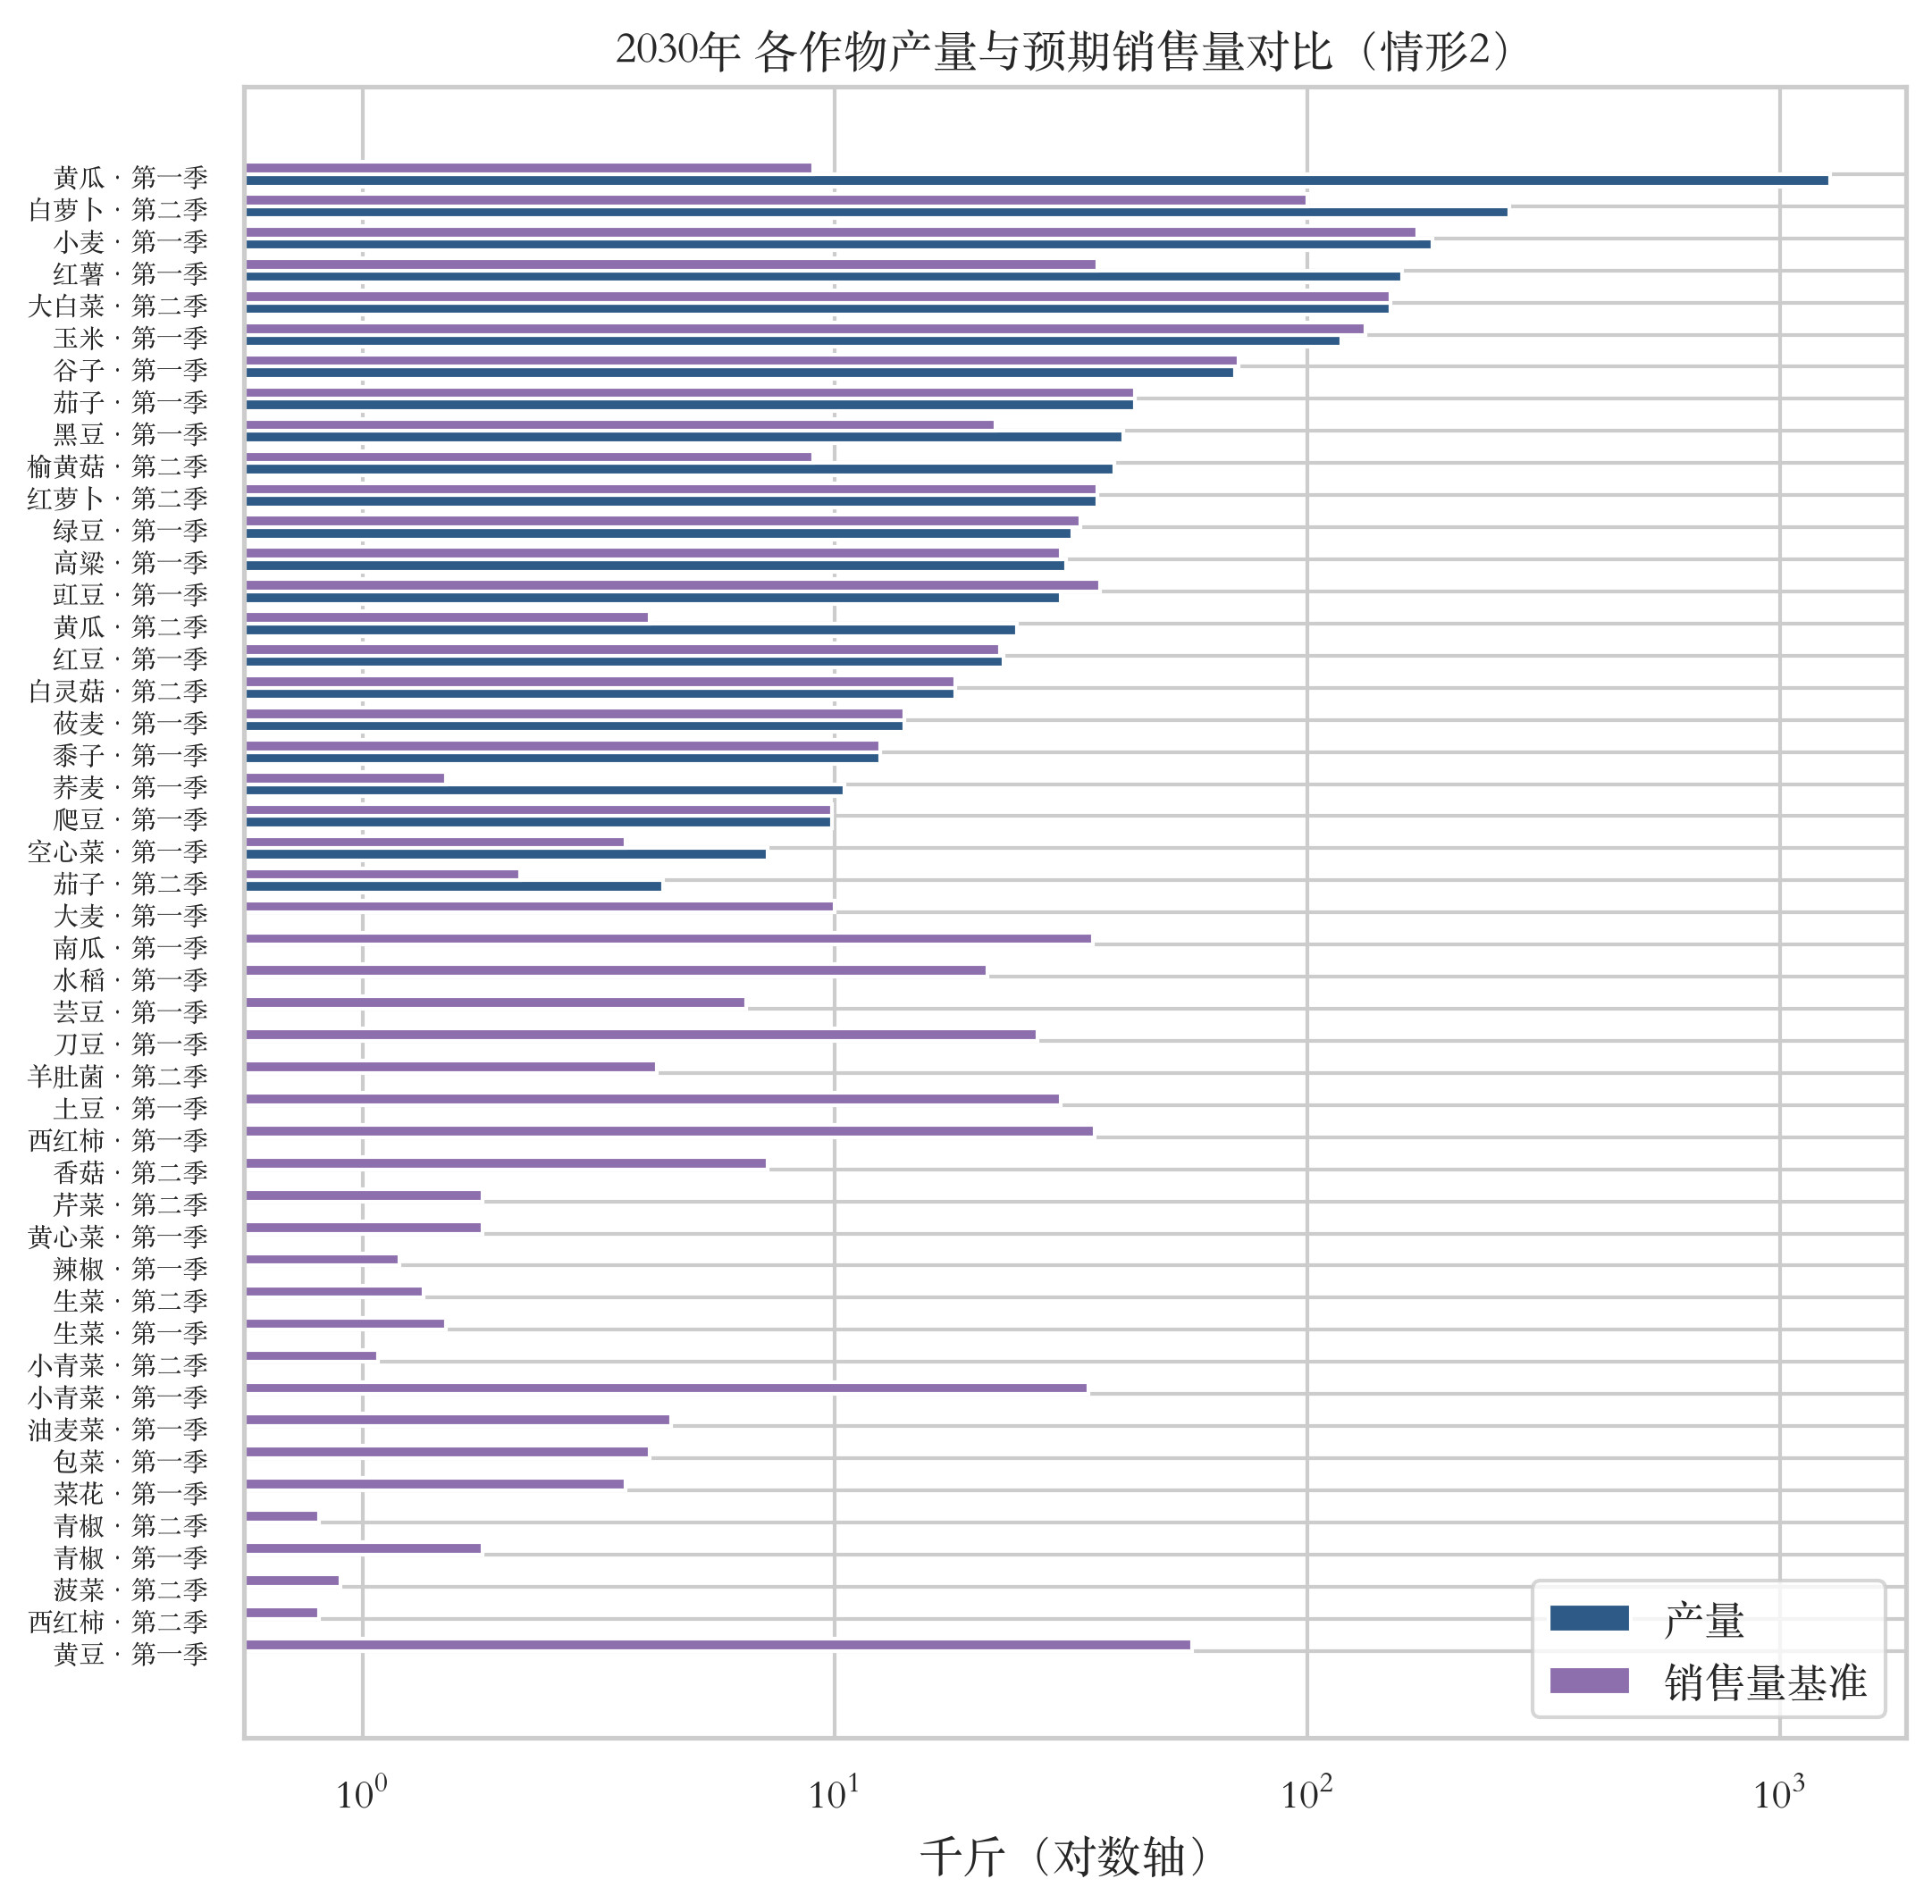
\includegraphics[width=0.78\textwidth]{figures/fig_prod_vs_sales_q1_2.png}
	\caption{情形2各作物产量与预期销售量对比}
	\label{fig:prod-vs-sales-q1-2}
\end{figure}

情形2放宽了销售规则：超产部分可按2023年价格的50\%降价出售，因此如图~\ref{fig:prod-vs-sales-q1-2} 所示，模型大幅扩种边际利润高、半价出售仍有利可图的蔬菜作物。粮食类面积占比降至81.9\%，蔬菜类升至17.4\%，黄瓜、茄子、西红柿等高价蔬菜的单季产量成倍超过其预期销售量，超产部分以半价消化（全周期超产约占总产量的55.3\%）。这说明在"滞销浪费"转为"半价出售"后，销售上限的约束作用被显著放松，种植决策从"匹配需求"转向"充分供给"，总净收益因而提高约48.4\%。情形2的结果也提示：若实际允许超产折价销售，应同步考虑市场容量与价格冲击，避免过度依赖单一高价作物。

\subsection{问题二的模型建立与求解}
\subsubsection{具体分析}

问题二在问题一基础上引入不确定性：销售量（小麦、玉米逐年增长5\%--10\%，其余作物相对2023年波动$\pm$5\%）、亩产量（$\pm$10\%）、种植成本（每年增长5\%）、销售价格（粮食类保持2023年价格，蔬菜类每年增长5\%，食用菌类逐年下降1\%--5\%，其中羊肚菌每年下降5\%）。由于种植方案须在年初一次性确定、而收益取决于当年市场与气候实现，这是典型的\textbf{两阶段随机规划}问题\cite{stochcrop1991,scenwp2008}：第一阶段决策（种植方案）为"现在定"，第二阶段决策（实际销售分配）为"看天吃饭"。同时，题目要求"总收益尽量大、风险尽量小"，需在期望收益与风险之间权衡，故引入条件风险价值（CVaR）度量尾部损失\cite{cvar2000,cvar2002}。

\subsubsection{不确定性建模与情景生成}

将第 $\omega$ 个随机情景下的参数记为：销售量乘子 $\tilde{m}^S_{\omega,c,s,t}$、亩产量乘子 $\tilde{m}^y_{\omega,c,t}$、价格 $\tilde{r}_{\omega,c,t}$、成本 $\tilde{c}_{c,p,s,t}$。题目只给出各参数相对2023年的波动区间而未给分布。为保证问题3在引入作物间相关时不改变各作物边际波动范围，两问对每作物的冲击统一采用截断标准正态 $\varepsilon\sim N(0,1)\cap[-1,1]$ 抽样，波动幅度均落在题目给定区间内：

\begin{equation}
\resizebox{0.98\textwidth}{!}{$\displaystyle
\tilde{m}^y_{\omega,c,t} = 1 + 0.10\,\varepsilon^y_{\omega,c},\qquad
\tilde{m}^S_{\omega,(c,s),t} = \begin{cases} (1+g)^{t-2023}, & g=\max\big(0.05,\ \min(0.10,\ 0.075+0.025\,\varepsilon^S_{\omega,(c,s)})\big),\ c\in\{\text{小麦,玉米}\}\\ 1+0.05\,\varepsilon^S_{\omega,(c,s)}, & \text{其他作物} \end{cases}
$}
\label{eq:uncert}
\end{equation}

\begin{equation}
\resizebox{0.98\textwidth}{!}{$\displaystyle
\tilde{r}_{\omega,c,t} = r_{c,s}\cdot \begin{cases} 1.05^{t-2023}\,(1+0.03\,\varepsilon^p_{\omega,c}), & \text{蔬菜}\\ 1+0.02\,\varepsilon^p_{\omega,c}, & \text{粮食}\\ 0.97^{t-2023}\,(1+0.02\,\varepsilon^p_{\omega,c}), & \text{其他食用菌}\\ 0.95^{t-2023}, & c=\text{羊肚菌} \end{cases},\qquad
\tilde{c}_{c,p,s,t}=c_{c,p,s}\times1.05^{t-2023}\,(1+0.05\,\varepsilon^c_{\omega,c})
$}
\label{eq:priceuncert}
\end{equation}

即：小麦、玉米销售量按年增长率 $g\in[0.05,0.10]$ 逐年累积，其余作物销售量相对2023年基准波动 $\pm5\%$；亩产量波动 $\pm10\%$；蔬菜价格在逐年上涨 $5\%$ 的基础上波动 $\pm3\%$，粮食价格保持2023年水平、仅波动 $\pm2\%$，食用菌价格按题目给定幅度逐年下降（羊肚菌 $-5\%$、其余 $-3\%$）；成本在逐年上涨 $5\%$ 的基础上波动 $\pm5\%$。用蒙特卡洛方法抽样 $N=30$ 个等概率情景近似随机变量的联合分布。问题2中各作物冲击相互独立；问题3将同一组冲击经 Cholesky 相关化，故两问边际分布完全一致、仅相关结构不同，可干净地分离"作物间相关性"对组合风险的净效应。

\subsubsection{两阶段随机规划模型}

种植决策 $x_{p,t,s,c}$ 为第一阶段变量（对全部情景一致，即"now"决策）；原价售出量 $u_{\omega,c,s,t}$ 为第二阶段变量，仅约束于对应情景。与问题1情形1一致，采用"超产滞销"规则：超出预期销售量的部分无法售出、不计收益。情景 $\omega$ 下的净收益为

\begin{equation}
\Pi_\omega = \sum_{c,s,t} \tilde{r}_{\omega,c,t}\, u_{\omega,c,s,t} - \sum_{p,t,s,c} \tilde{c}_{c,p,s,t} A_p x_{p,t,s,c}
\label{eq:profit-scen}
\end{equation}

产量-销售关系约束（逐情景）为 $u_{\omega,c,s,t}\le \sum_p A_p \tilde{m}^y_{\omega,c,t} y_{c,p,s}x_{p,t,s,c}$（售出量不超过产量）、$u_{\omega,c,s,t}\le \tilde{m}^S_{\omega,c,s,t}S_{c,s}$（不超过情景销售量）。亩产量的随机波动刻画了气候等自然因素对产量的影响\cite{climate2009}。

考虑风险的目标函数采用"期望收益 $-$ $\lambda\cdot$ CVaR"形式：

\begin{equation}
\max\quad \mathbb{E}_\omega[\Pi_\omega] - \lambda\, \mathrm{CVaR}_\alpha(-\Pi_\omega)
\label{eq:obj3}
\end{equation}

其中 $-\Pi_\omega$ 为情景损失。参照 Rockafellar--Uryasev 的线性化公式\cite{cvar2000,cvar2002}，引入辅助变量 $\eta$ 与 $\zeta_\omega$：

\begin{equation}
\mathrm{CVaR}_\alpha(-\Pi_\omega) = \eta + \frac{1}{(1-\alpha)|\Omega|}\sum_{\omega\in\Omega}\zeta_\omega, \qquad
\zeta_\omega \ge -\Pi_\omega - \eta,\ \zeta_\omega\ge 0
\label{eq:cvar-linear}
\end{equation}

置信水平取 $\alpha=0.90$，即考察最差10\%情景（$N=30$ 时对应最差3个情景）的平均损失。风险系数 $\lambda$ 度量决策者对风险的厌恶程度：$\lambda=0$ 退化为纯期望收益最大化，$\lambda$ 增大则方案更保守。通过求解不同 $\lambda$ 下的模型，可得到收益-风险前沿，供决策者选择。约束（式\ref{eq:c1}--\ref{eq:c5}）在随机框架下全部保留（销售上限改为逐情景形式）。

\subsubsection{模型求解}

抽样 $N=30$ 个等概率情景，取相对最优间隙 $4\%$、置信水平 $\alpha=0.90$，分别以 $\lambda=0,0.3,0.6,0.9$ 求解，得到不同风险偏好下的最优种植方案与风险指标（期望收益、标准差、最差情景收益、CVaR、亏损概率）。求解采用 HiGHS 分支定界，并以问题1的可行方案作 MIP 热启动以加速收敛。求解结果见问题二结果分析部分。

\subsection{问题三的模型建立与求解}
\subsubsection{具体分析}

问题二假设各作物不确定性相互独立，但现实中作物间存在明显关联：消费者常在相近菜品间替代（如大白菜与白萝卜、小麦与玉米），也常搭配购买（如粮食与蔬菜、蔬菜与食用菌）；同时销售价格与销售量负相关、亩产量与价格负相关、亩产量与销售量正相关。忽略这些关联会低估方案的真实风险。问题三据此构造相关性矩阵 $\Sigma$，用 Cholesky 分解生成相关情景，在相关口径下重新优化并对比。

\subsubsection{相关结构建模}

定义随机向量 $\boldsymbol{\xi}$ 由四部分构成：47个销售冲击 $\varepsilon_{(c,s)}$、41个产量冲击 $\delta_c$、41个价格冲击 $\pi_c$、41个成本冲击 $\chi_c$，共170维。相关性矩阵 $\Sigma$ 按以下逻辑设定：

\begin{itemize}
	\item \textbf{共同因子}：全部41种作物产量的天气共同因子（$\rho=+0.35$，同一区域丰歉同向）、蔬菜价格的共同市场因子（$\rho=+0.25$）、成本共同因子（$\rho=+0.15$）；
	\item \textbf{替代组}（销售量负相关，两作物组 $\rho=-0.6$、多作物组星形 $\rho=-0.4$）：小麦--玉米、大白菜--白萝卜--红萝卜、黄豆--黑豆--红豆--绿豆--爬豆、豇豆--刀豆--芸豆、四种食用菌、西红柿--青椒--辣椒等互为替代的作物组；
	\item \textbf{互补组}（销售量正相关 $\rho=+0.4$）：粮食与蔬菜、蔬菜与食用菌等搭配消费的作物对；
	\item \textbf{产销联动}：销售量--价格 $\rho=-0.5$（供给增加压价）、产量--价格 $\rho=-0.3$（丰产降价）、产量--销售量 $\rho=+0.2$（丰产多销）。
\end{itemize}

目标矩阵可能不满足半正定性，用 Higham 交替投影\cite{higham2002}将其投影到"单位对角 $+$ 半正定"的最近相关矩阵，再用 \textbf{Cholesky 分解} $\Sigma = LL^{\top}$ 生成相关标准正态向量 $\mathbf{z}=L\boldsymbol{\xi}_0$（$\boldsymbol{\xi}_0$ 为标准正态白噪声，$\mathbf{z}$ 各分量截断到 $[-1,1]$ 以保证波动幅度不越界），映射回销量/产量/价格/成本乘子得到相关情景：

\begin{equation}\label{eq:cholesky}
\resizebox{0.96\textwidth}{!}{$\displaystyle
\begin{aligned}
\tilde{m}^y_{\omega,c,t}&=1+0.10\,z_{c},\qquad
\tilde{m}^S_{\omega,(c,s),t}=\begin{cases}(1+g)^{t-2023}, & g=\max\big(0.05,\ \min(0.10,\ 0.075+0.025z_{c,s})\big)\\ 1+0.05z_{c,s}, & \text{其他作物}\end{cases},\\
\tilde{r}_{\omega,c,t}&=r_{c,s}\times\begin{cases}1.05^{t-2023}(1+0.03z_{c}), & \text{蔬菜}\\ 1+0.02z_{c}, & \text{粮食}\\ 0.97^{t-2023}(1+0.02z_{c}), & \text{其他食用菌}\\ 0.95^{t-2023}, & \text{羊肚菌}\end{cases},\quad
\tilde{c}_{c,p,s,t}=c_{c,p,s}\times1.05^{t-2023}(1+0.05z_{c})
\end{aligned}
$}
\end{equation}

\subsubsection{求解与对比}

将相关情景代入问题二的两阶段随机规划模型（目标式\ref{eq:obj3}），在相同 $\lambda$ 下重新求解，并与独立情景结果对比。理论上，替代效应使同组作物"此消彼长"，组合种植可对冲个别作物销售不及预期的风险；互补效应则放大同涨同跌，使整体收益波动增大。通过对比相关与独立两种口径下的期望收益、标准差与CVaR，可定量说明相关性对种植策略的影响并论证方案调整的合理性，结果见问题三结果分析部分。

\subsection{问题二结果分析}

取 $N=30$ 个情景、随机种子2024、$\alpha=0.90$、相对最优间隙 $4\%$，分别以 $\lambda=0,0.3,0.6,0.9$ 求解，各风险偏好下的最优方案与风险指标见表\ref{tab:q2scan}。

\begin{table}[htbp]
	\caption{问题2 不同风险系数下的最优方案指标（$N=30$）}
	\label{tab:q2scan}
	\centering
	\begin{tabular}{ccccc}
		\toprule
		$\lambda$ & 期望收益(万元) & 标准差(万元) & 最差情景(万元) & CVaR短缺口(万元) \\
		\midrule
		0 & 4022.3 & 56.2 & 3874.0 & 104.8 \\
		0.3 & 4022.3 & 56.2 & 3874.0 & 104.8 \\
		0.6 & 4022.3 & 56.2 & 3874.0 & 104.8 \\
		0.9 & 4022.3 & 56.2 & 3874.0 & 104.8 \\
		\bottomrule
	\end{tabular}
\end{table}

结果表明：独立情景下期望收益约 $4\,022.3$ 万元，标准差仅 $56.2$ 万元（相对期望 $1.40\%$），最差情景收益 $3\,874.0$ 万元（偏离期望 $3.69\%$），CVaR短缺口（期望收益减最差 $10\%$ 情景平均收益）约 $104.8$ 万元，任何情景均不亏损。与问题1情形1的确定性结果 $3\,988.2$ 万元相比，期望收益略高约 $0.9\%$，主要来自蔬菜价格逐年上涨等确定性趋势，而非随机波动的有利实现。

一个值得注意的现象是：四组 $\lambda$ 得到完全相同的种植方案与风险指标，收益-风险前沿退化为一点（图\ref{fig:q23-lambda}）。其原因在于独立情景下各作物风险彼此无关，组合已通过品种多样化充分分散了可对冲的个体风险，剩余波动主要来自各作物自身的边际波动（产量 $\pm10\%$ 等）在有限情景下的叠加，其大小与种植结构关系不大，故改变风险厌恶程度几乎不改变最优方案。图\ref{fig:scen-dist-q2} 的情景收益分布印证了这一点：30个情景的收益分布窄而集中，标准差仅约 $56$ 万元。

\begin{figure}[htbp]
	\centering
	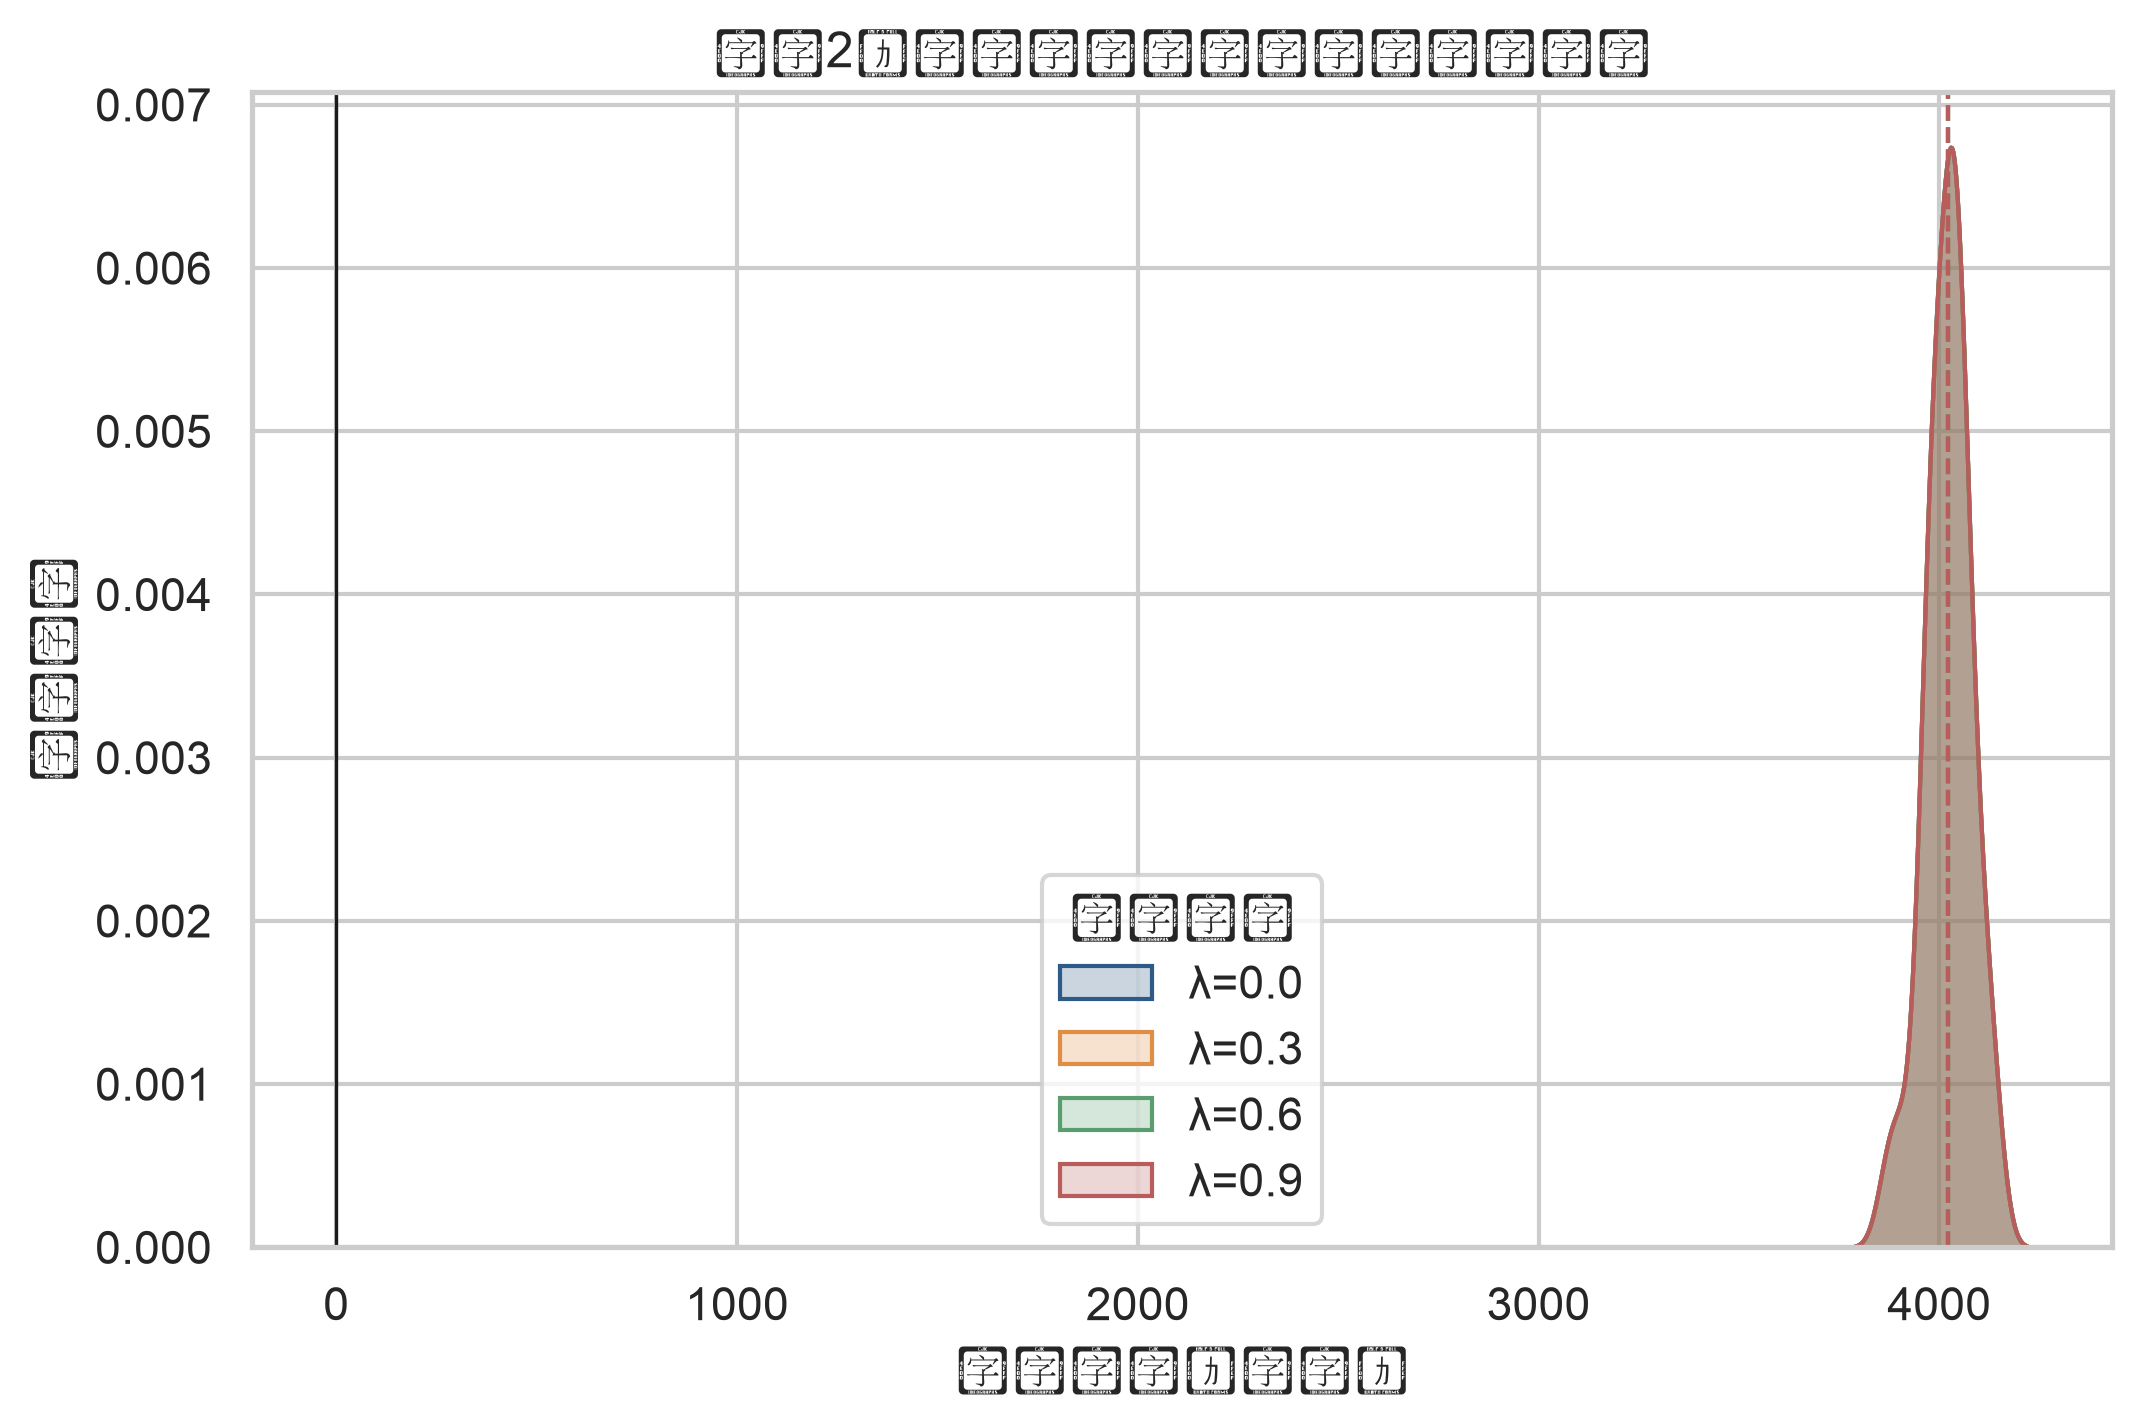
\includegraphics[width=0.68\textwidth]{figures/fig_scen_dist_q2.png}
	\caption{问题2 情景收益分布}
	\label{fig:scen-dist-q2}
\end{figure}

\begin{figure}[htbp]
	\centering
	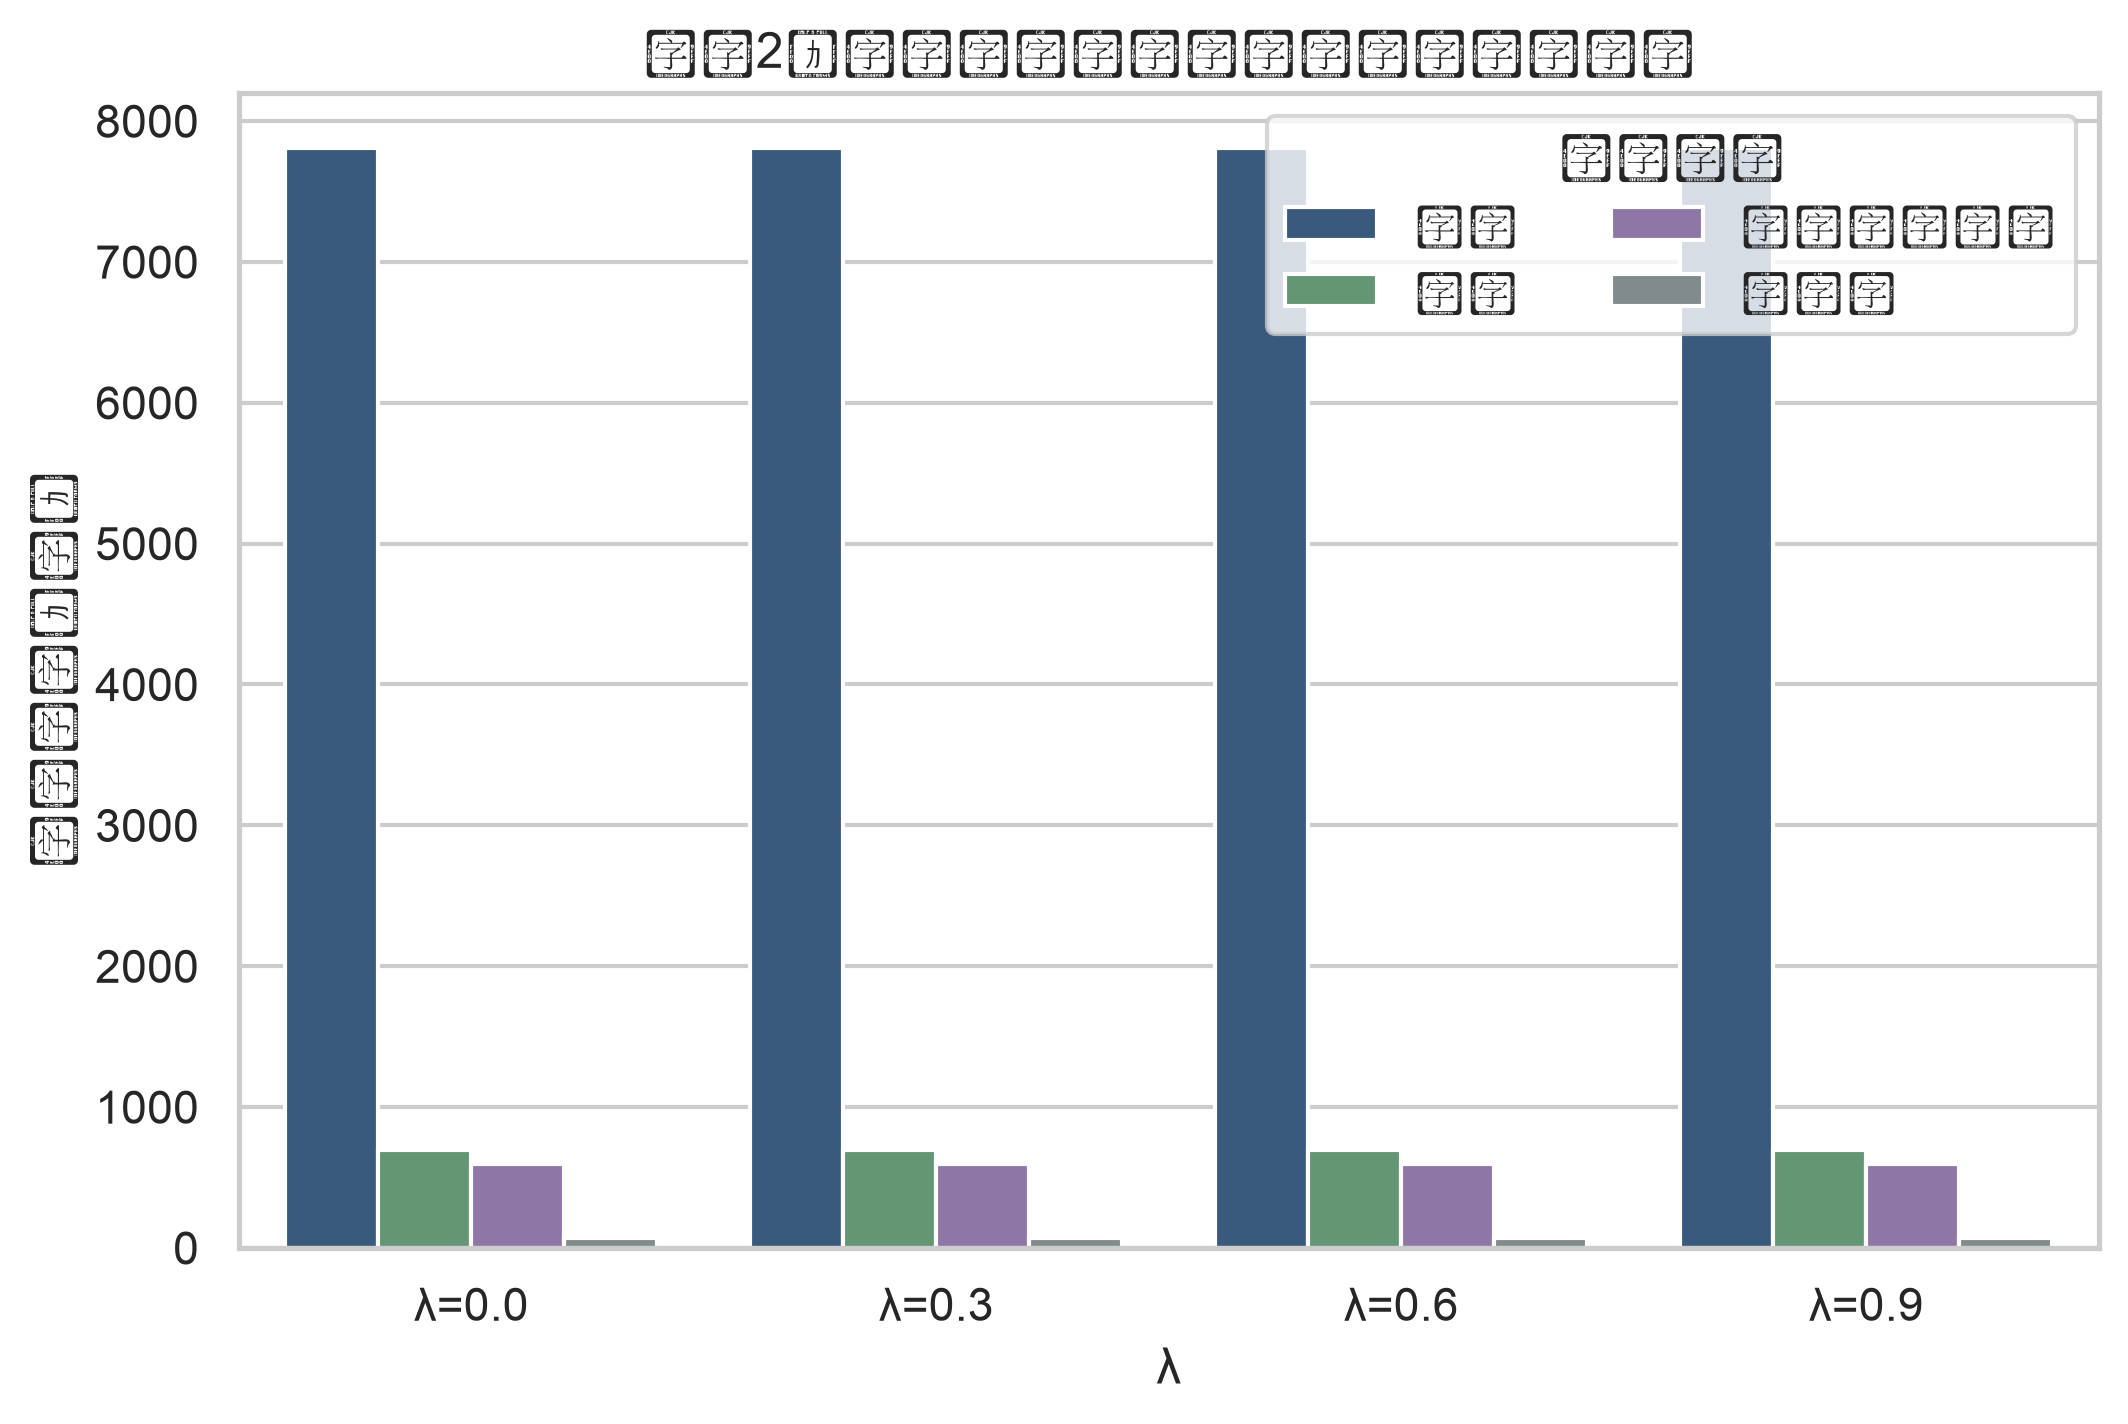
\includegraphics[width=0.78\textwidth]{figures/fig_area_q2.png}
	\caption{问题2 各年种植面积结构}
	\label{fig:area-q2}
\end{figure}

\subsection{问题三结果分析}

将相关情景代入同一随机规划模型，取 $N=30$、种子7、$\alpha=0.90$，同样以 $\lambda=0,0.3,0.6,0.9$ 求解，结果见表\ref{tab:q3scan}。

\begin{table}[htbp]
	\caption{问题3 不同风险系数下的最优方案指标（$N=30$）}
	\label{tab:q3scan}
	\centering
	\begin{tabular}{ccccc}
		\toprule
		$\lambda$ & 期望收益(万元) & 标准差(万元) & 最差情景(万元) & CVaR短缺口(万元) \\
		\midrule
		0 & 4019.3 & 98.9 & 3836.3 & 173.8 \\
		0.3 & 4019.3 & 98.9 & 3836.3 & 173.8 \\
		0.6 & 4019.3 & 98.9 & 3836.3 & 173.8 \\
		0.9 & 4019.3 & 98.9 & 3836.3 & 173.8 \\
		\bottomrule
	\end{tabular}
\end{table}

与问题2相比，期望收益几乎不变（$4\,019.3$ 万元 vs $4\,022.3$ 万元，差 $0.07\%$），但组合风险系统性抬升：收益标准差由 $56.2$ 万元（$1.40\%$）升至 $98.9$ 万元（$2.46\%$，约 $1.76$ 倍），最差情景偏离期望由 $3.69\%$ 扩大至 $4.55\%$，CVaR短缺口由 $104.8$ 万元升至 $173.8$ 万元（约 $1.66$ 倍）。图\ref{fig:q23-dist} 的情景收益分布对比直观显示：相关情景下分布明显展宽、左尾加长；图\ref{fig:q23-risk} 从标准差、最差偏离与CVaR短缺口三个维度一致说明"考虑相关性后组合风险显著放大"。跨3组随机种子（问题2用种子2024/2025/2026、问题3用7/8/9）复核后，问题3的标准差与CVaR短缺口均一致高于问题2（详见模型检验与分析一节），结论方向稳健。

\begin{figure}[htbp]
	\centering
	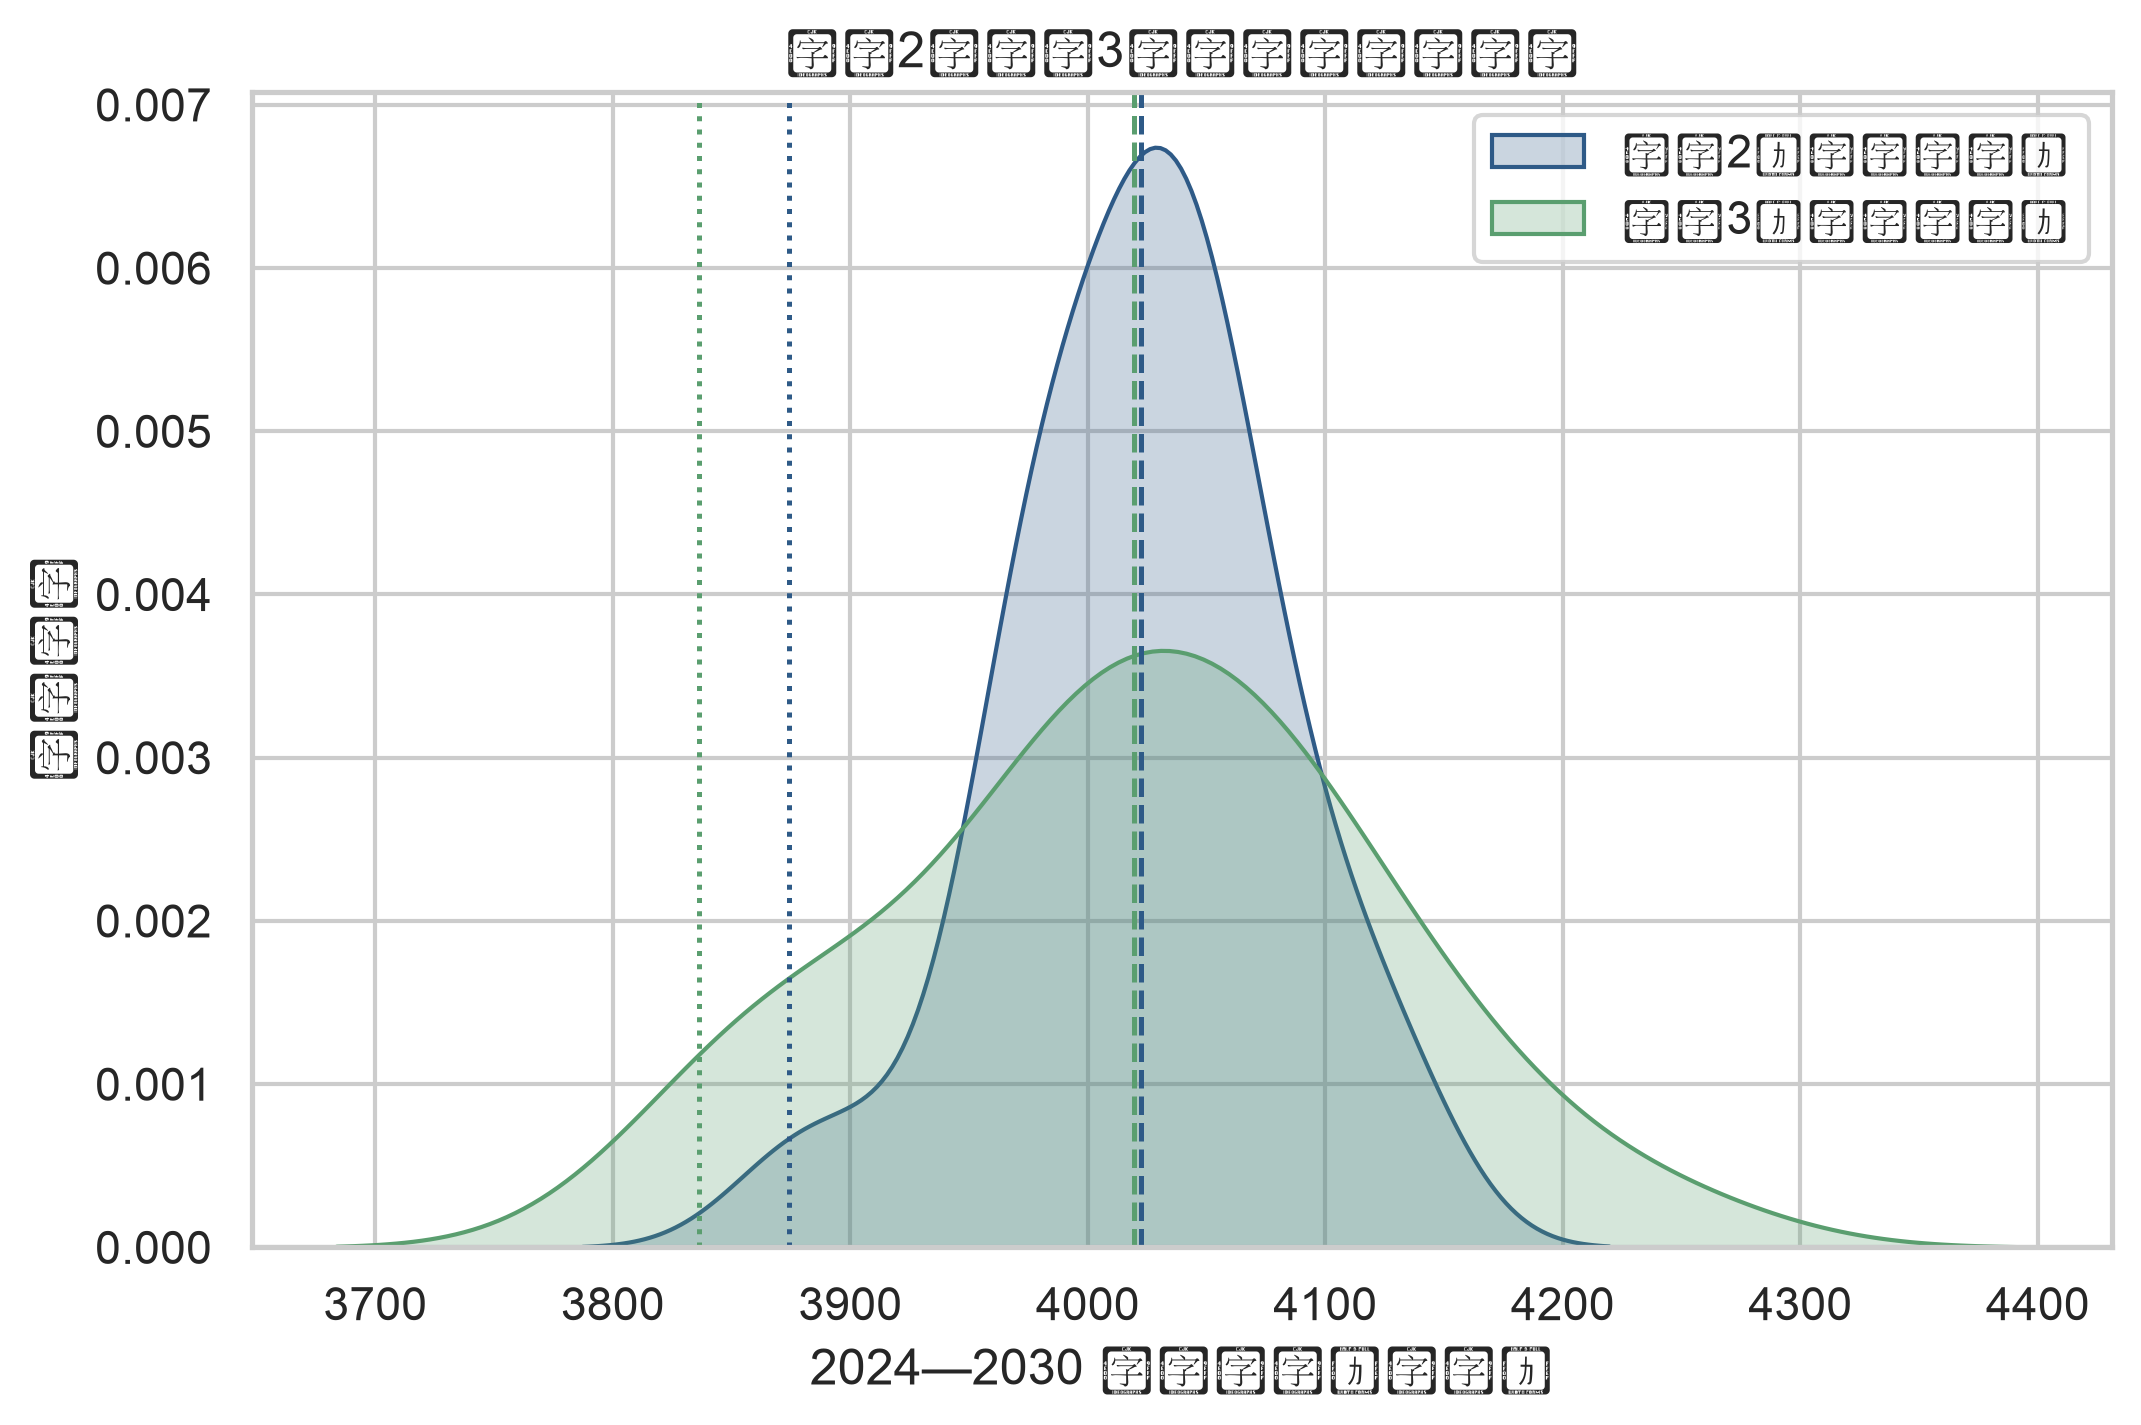
\includegraphics[width=0.80\textwidth]{figures/fig_q23_dist.png}
	\caption{问题2与问题3情景收益分布对比}
	\label{fig:q23-dist}
\end{figure}

\begin{figure}[htbp]
	\centering
	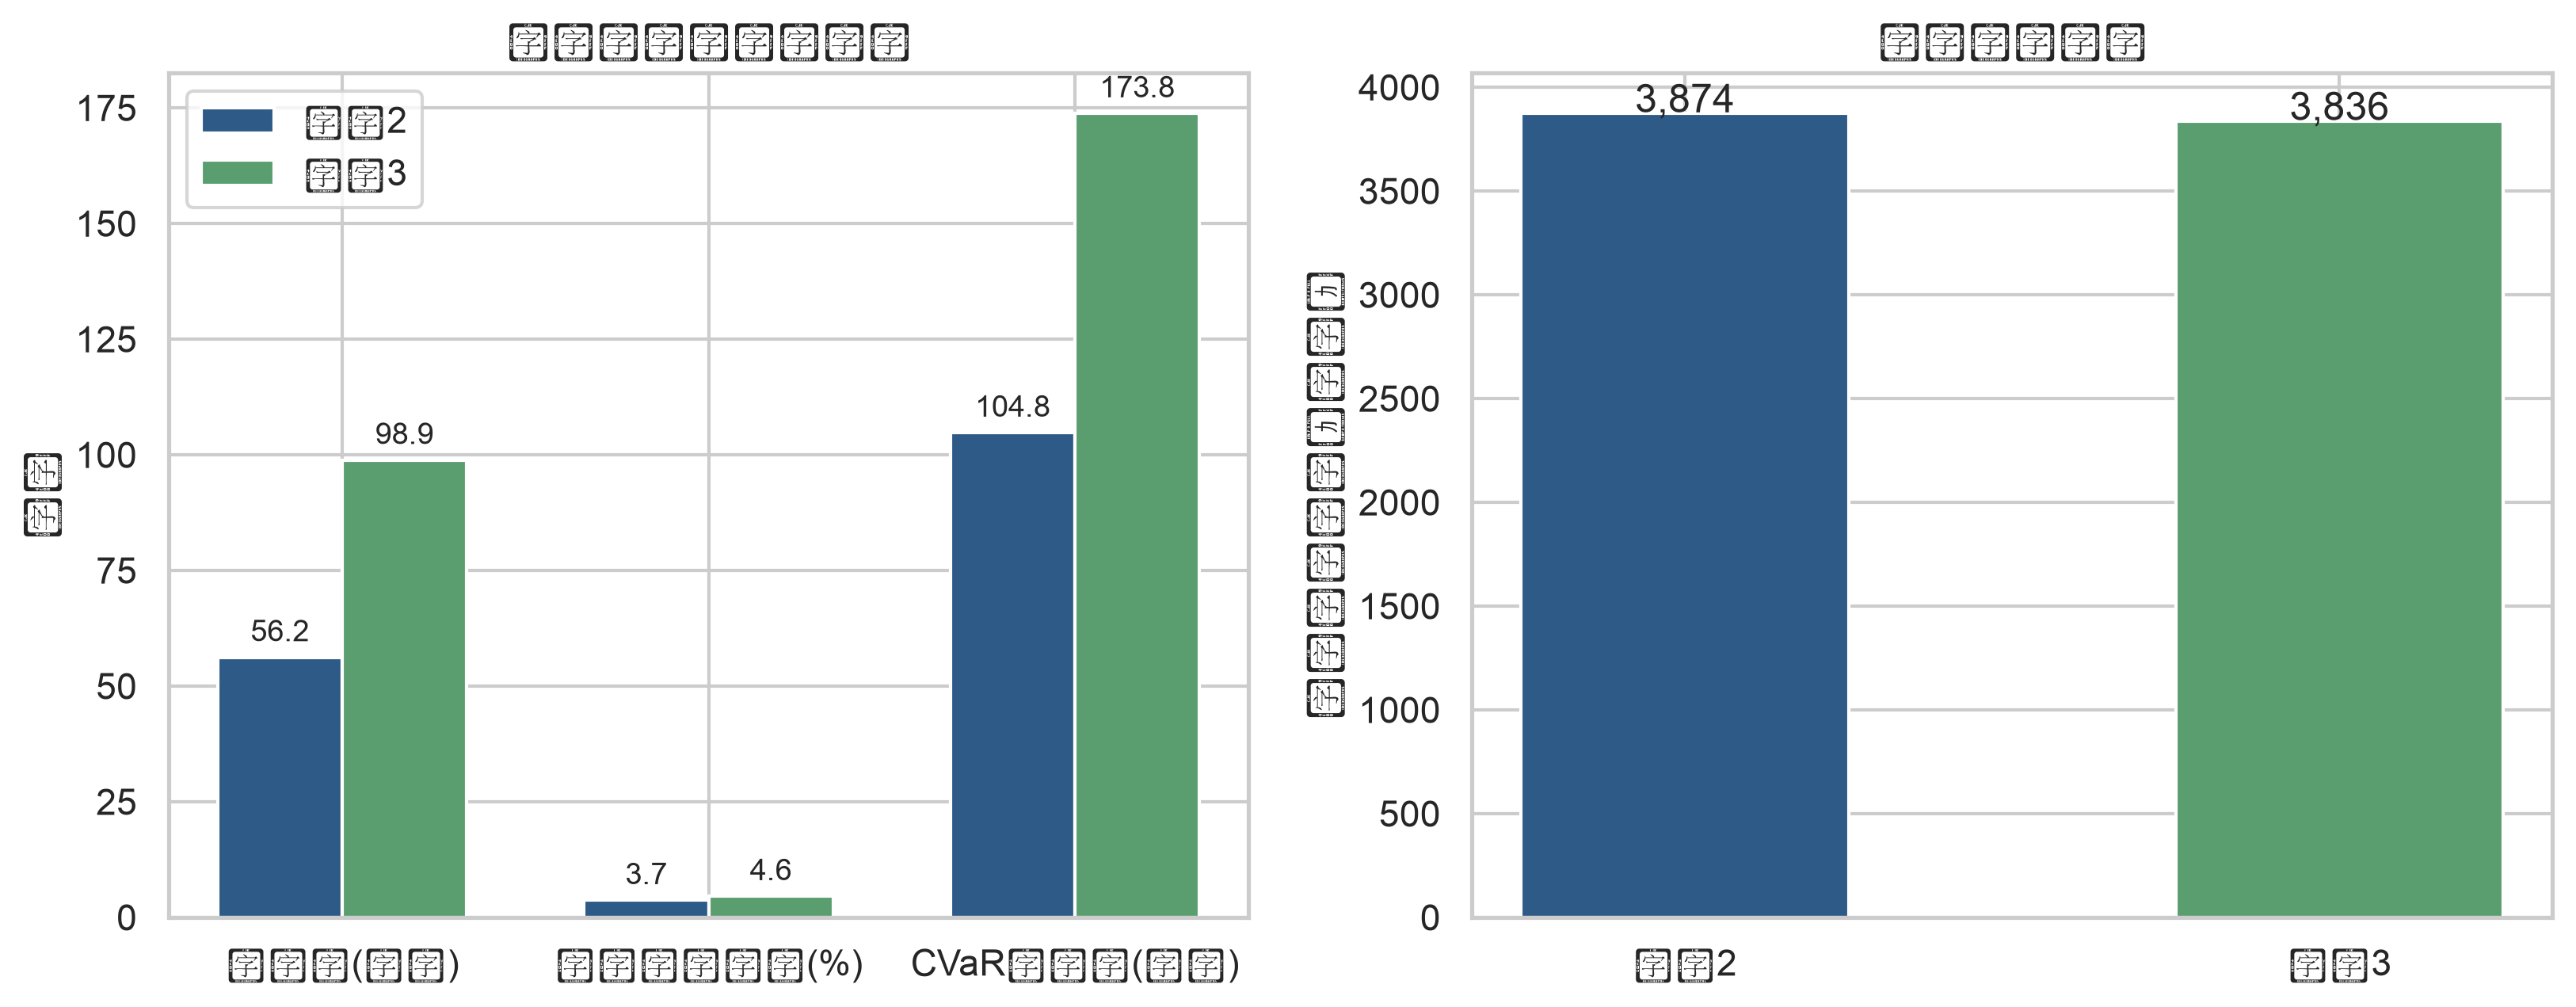
\includegraphics[width=0.90\textwidth]{figures/fig_q23_risk.png}
	\caption{相关性对组合风险指标的影响}
	\label{fig:q23-risk}
\end{figure}

\begin{figure}[htbp]
	\centering
	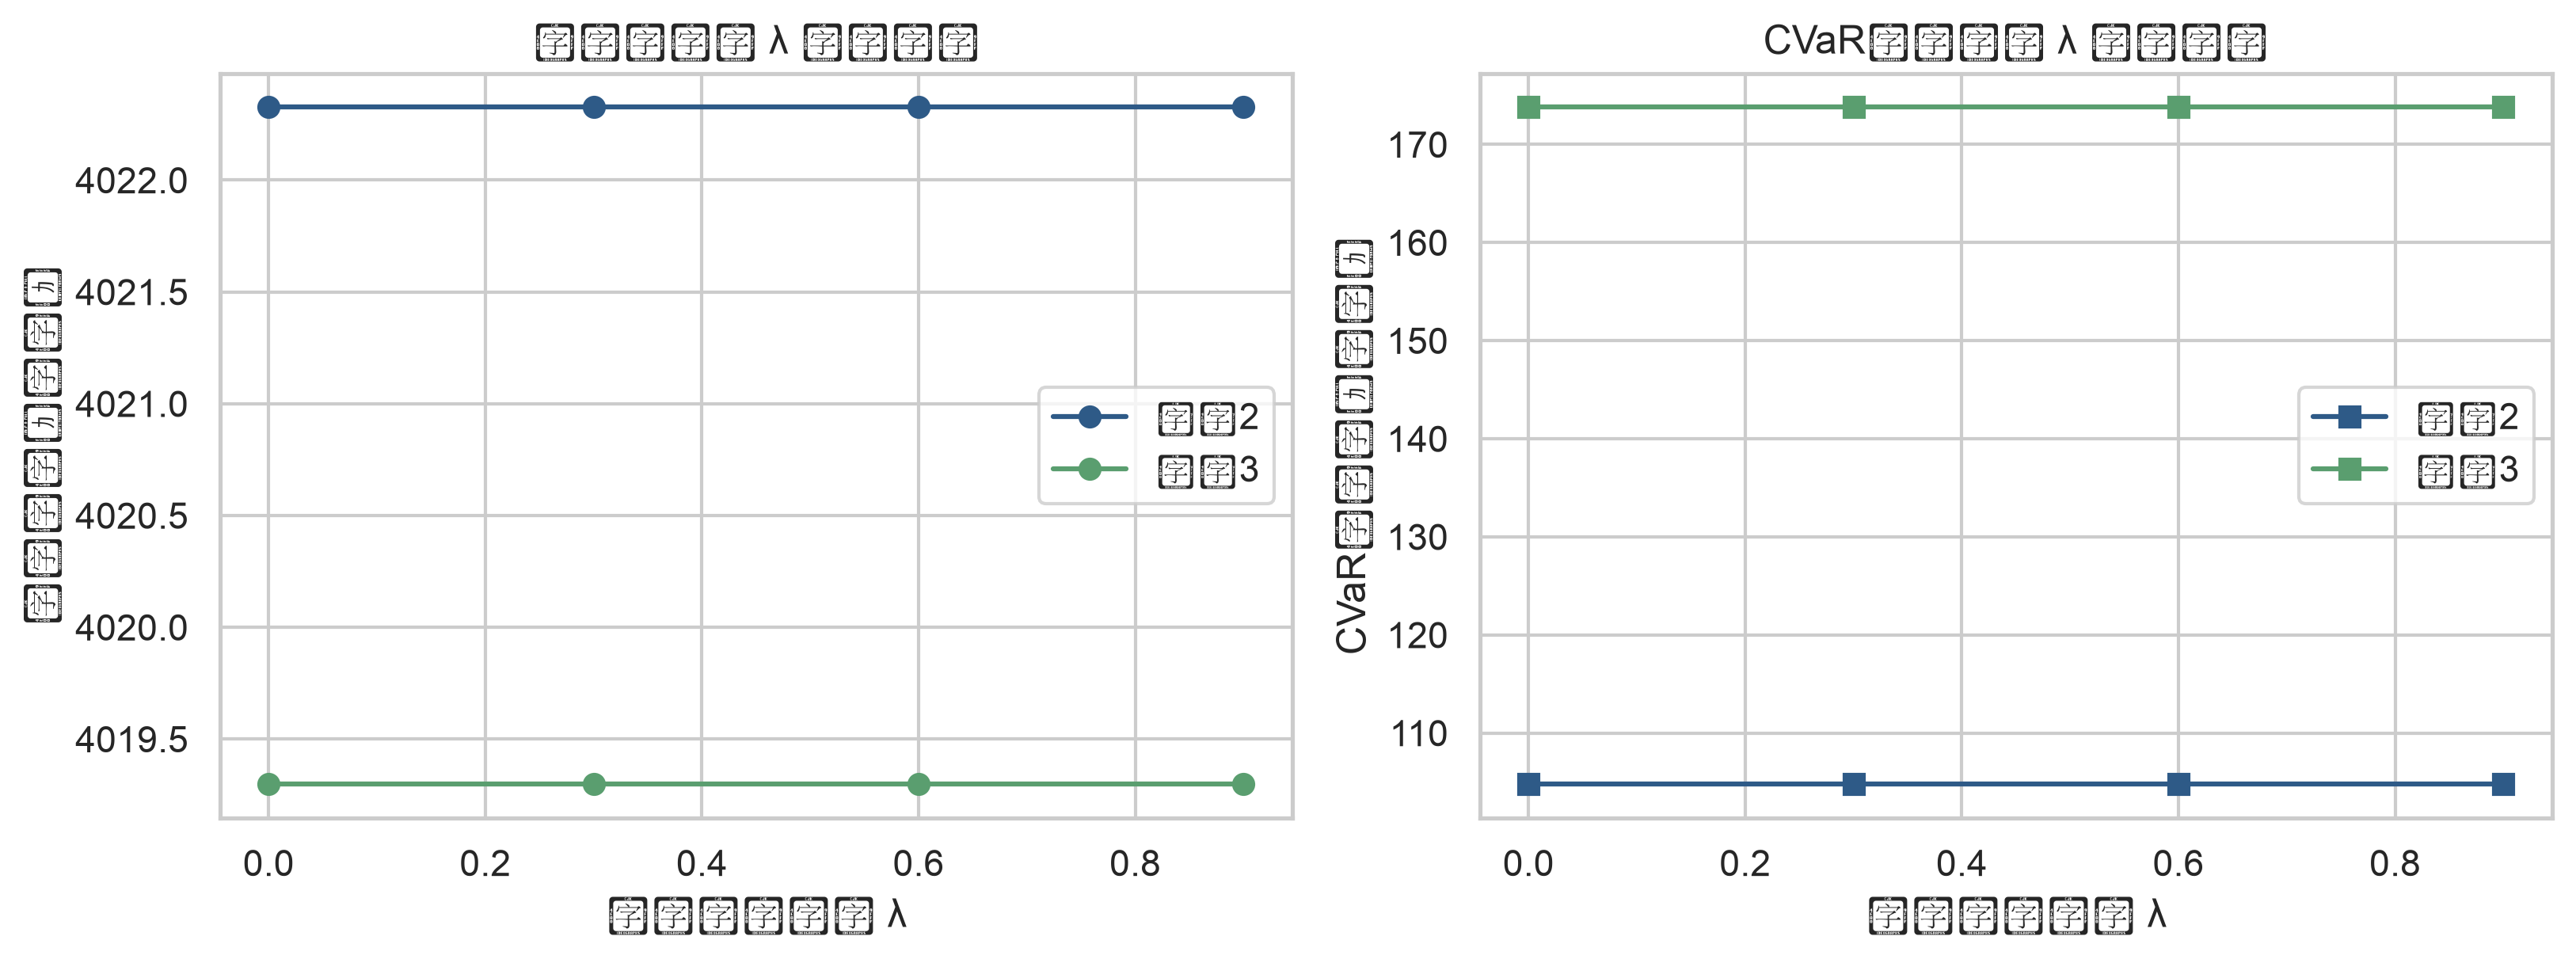
\includegraphics[width=0.90\textwidth]{figures/fig_q23_lambda.png}
	\caption{期望收益与CVaR短缺口对风险系数$\lambda$的敏感性}
	\label{fig:q23-lambda}
\end{figure}

风险放大的机制可定量解释。问题3的相关矩阵保留了三个共同因子：全部41种作物产量的天气因子（相关 $0.35$）、蔬菜价格的共同市场因子（$0.25$）与成本共同因子（$0.15$）。共同因子使不利事件（歉收、菜价下跌、成本上升）在作物间同步发生，组合无法通过多样化对冲，直接放大尾部损失；替代组（小麦--玉米 $-0.55$、大白菜--白萝卜--红萝卜 $-0.40$ 等）虽使同组作物"此消彼长"、提供部分对冲，但仅覆盖少数销售组合，不足以抵消共同因子主导的风险放大。这解释了为什么相关情景下组合风险约为独立情景的 $1.7$ 倍。

值得注意的是，虽然风险显著放大，相关与独立两种口径下的最优种植方案几乎一致（$564$ 个地块种植决策中仅 $1$ 个不同），期望收益也几乎相同。这说明：在给定的边际波动幅度下，最优种植结构主要由各作物的收益-成本结构与轮作制度约束决定，对"作物间是否相关"这一联合分布假设不敏感；相关性主要作用于风险测度，而非方案本身。因此实际生产中即使无法精确估计作物间的相关强度，只要边际波动范围设定合理，本文推荐的种植结构依然稳健，但必须充分认识到其真实尾部风险高于"独立假设"下的估计。

\begin{figure}[htbp]
	\centering
	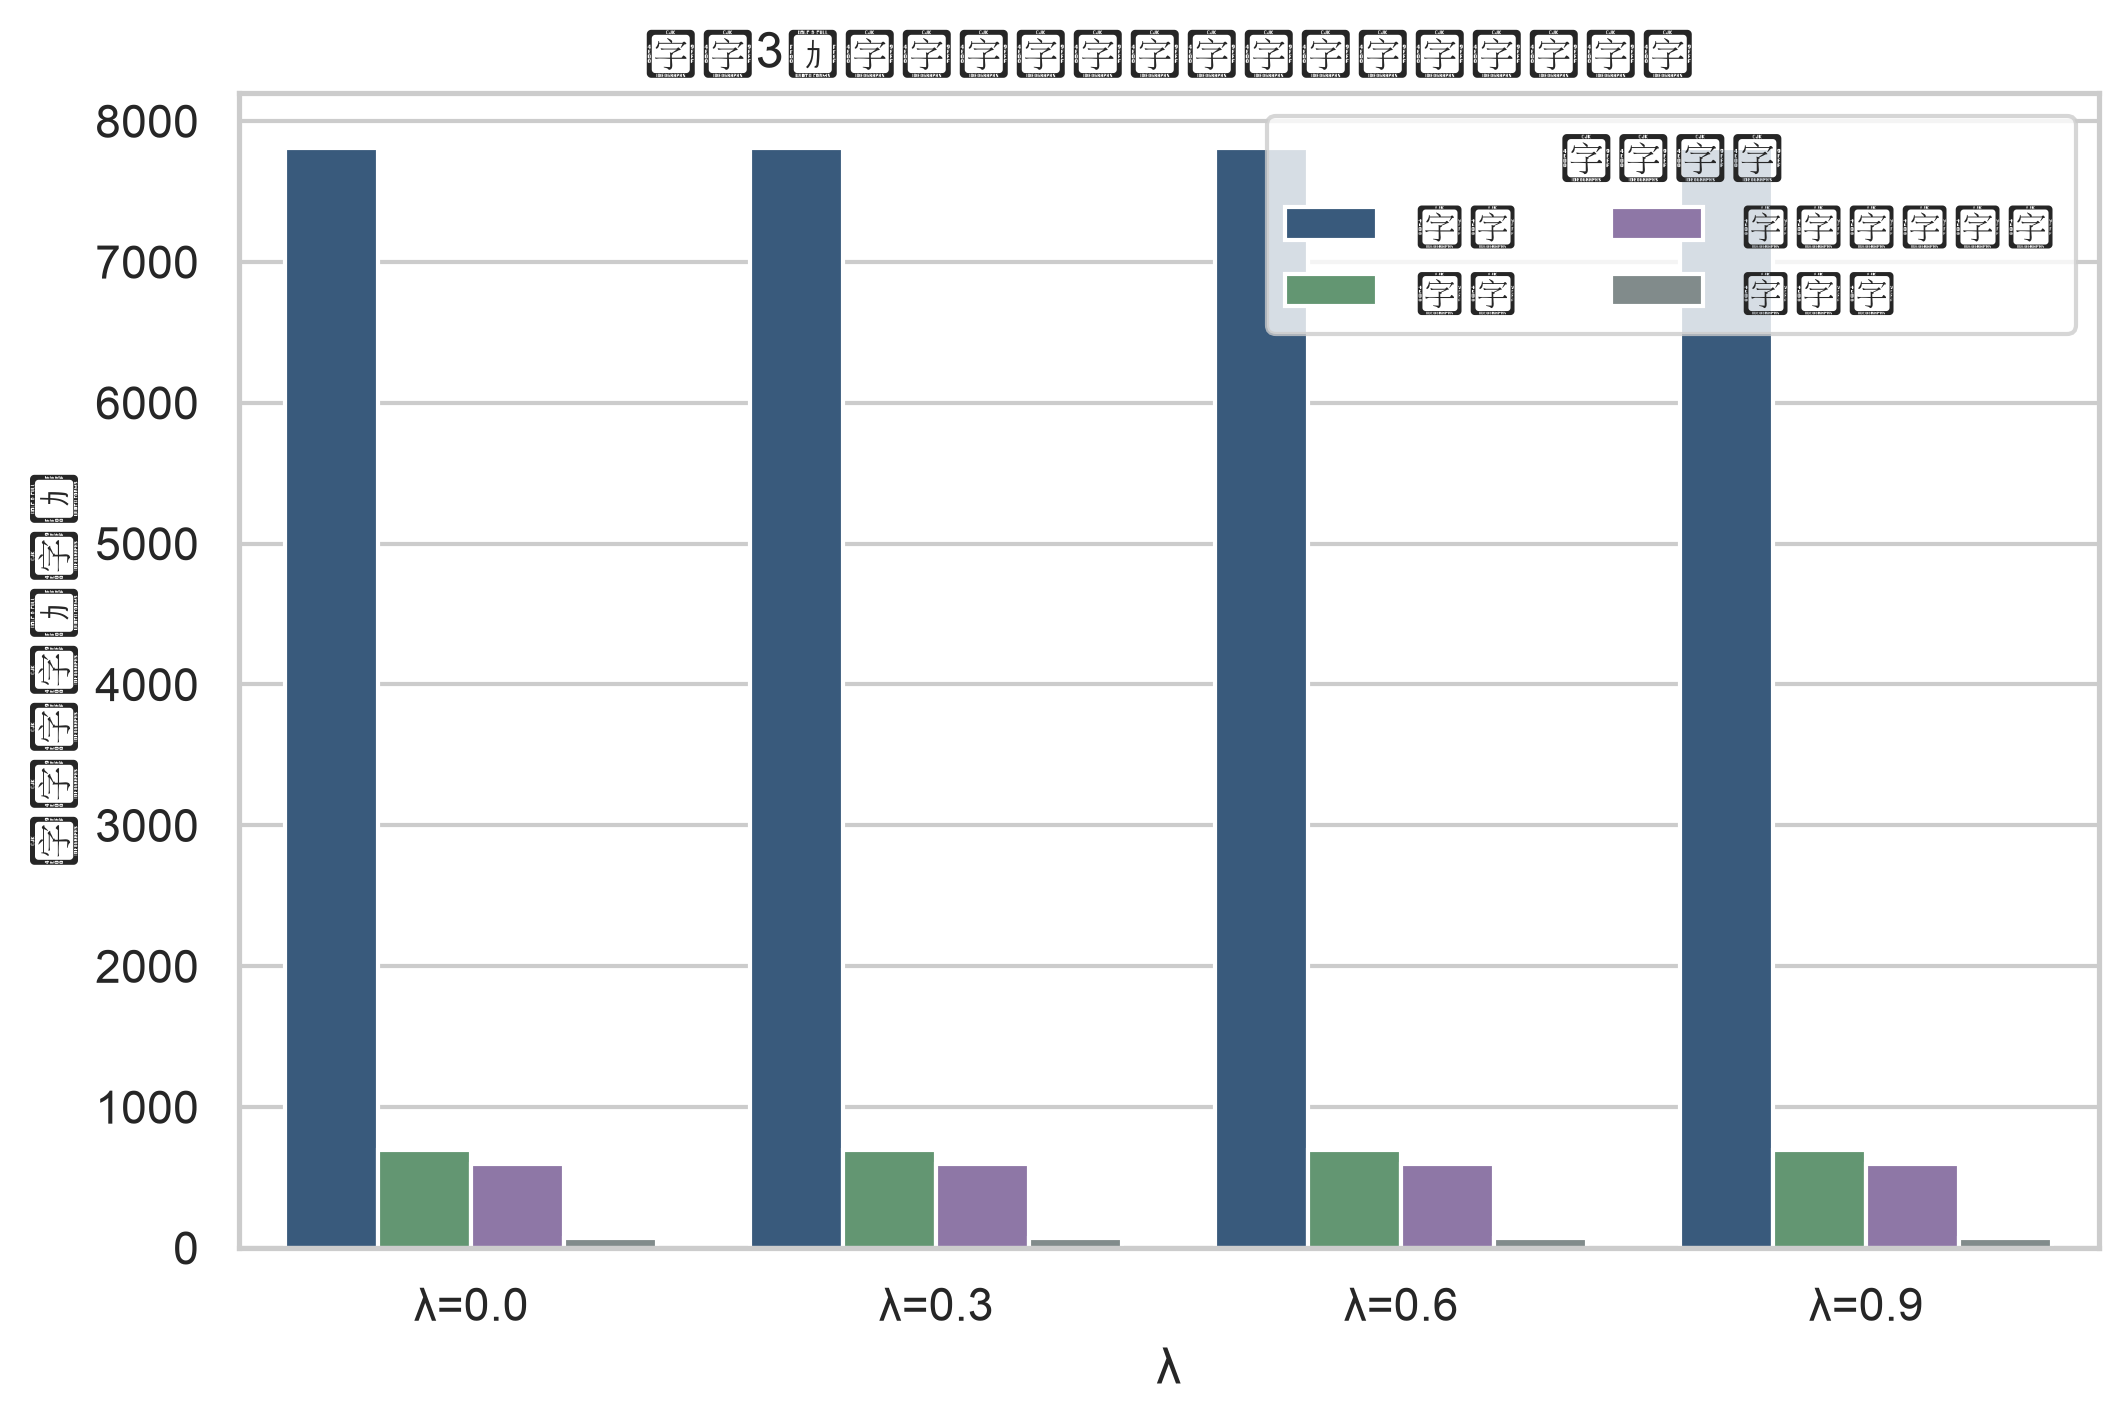
\includegraphics[width=0.78\textwidth]{figures/fig_area_q3.png}
	\caption{问题3 各年种植面积结构}
	\label{fig:area-q3}
\end{figure}
